% $Header: /cvsroot/latex-beamer/latex-beamer/solutions/generic-talks/generic-ornate-15min-45min.en.tex,v 1.4 2004/10/07 20:53:08 tantau Exp $

\documentclass{beamer}

% This file is a solution template for:

% - Giving a talk on some subject.
% - The talk is between 15min and 45min long.
% - Style is ornate.



% Copyright 2004 by Till Tantau <tantau@users.sourceforge.net>.
%
% In principle, this file can be redistributed and/or modified under
% the terms of the GNU Public License, version 2.
%
% However, this file is supposed to be a template to be modified
% for your own needs. For this reason, if you use this file as a
% template and not specifically distribute it as part of a another
% package/program, I grant the extra permission to freely copy and
% modify this file as you see fit and even to delete this copyright
% notice. 


\mode<presentation>
{
  \usetheme{Warsaw}
  % or ...

  \setbeamercovered{transparent}
  % or whatever (possibly just delete it)
}

\usepackage{pgf,pgfarrows,pgfnodes,pgfautomata,pgfheaps,pgfshade}
\usepackage[all,knot]{xy}
\usepackage[english]{babel}
% or whatever

\usepackage[latin1]{inputenc}
% or whatever

\usepackage{times}
\usepackage[T1]{fontenc}
% Or whatever. Note that the encoding and the font should match. If T1
% does not look nice, try deleting the line with the fontenc.

% \pgfdeclaremask{TrefoilAsDevice}{TrefoilMethodIllustration21072006}

% \pgfdeclareimage[interpolate=true,mask=TrefoilAsDevice,%
%                  width=1.8361cm,height=2cm]{trefoilimage}{beamer-trefoil}

% \newcommand{\putmachine}[2]{%
%   \pgfputat{#1}{\pgfbox[center,center]{\pgfuseimage{trefoilimage}}}%
%   \pgfputat{\pgfrelative{#1}{\pgfxy(0,-1.4)}}{\pgfbox[center,base]{\structure{#2}}}%
%   \pgfnodecircle{machine}[virtual]{\pgfrelative{#1}{\pgfxy(0,1)}}{2pt}%
% }

\usepackage {mathpartir}
\usepackage{bcprules}
%\usepackage{listings}


% Double brackets
\newcommand{\ldb}{[\![}
\newcommand{\rdb}{]\!]}
\newcommand{\ldrb}{(\!(}
\newcommand{\rdrb}{)\!)}
\newcommand{\lliftb}{\langle\!|}
\newcommand{\rliftb}{|\!\rangle}
% \newcommand{\lpquote}{\langle}
% \newcommand{\rpquote}{\rangle}
% \newcommand{\lpquote}{\lceil}
% \newcommand{\rpquote}{\rceil}
\newcommand{\lpquote}{\ulcorner}
\newcommand{\rpquote}{\urcorner}
\newcommand{\newkw}{\nu}

% SYNTAX
\newcommand{\id}[1]{\texttt{#1}}
\newcommand{\none}{\emptyset}
\newcommand{\eps}{\epsilon}
\newcommand{\set}[1]{\{#1\}}
\newcommand{\rep}[2]{\id{\{$#1$,$#2$\}}}
\newcommand{\elt}[2]{\id{$#1$[$#2$]}}
\newcommand{\infinity}{$\infty$}

\newcommand{\pzero}{\mathbin{0}}
\newcommand{\seq}{\mathbin{\id{,}}}
\newcommand{\all}{\mathbin{\id{\&}}}
\newcommand{\choice}{\mathbin{\id{|}}}
\newcommand{\altern}{\mathbin{\id{+}}}
\newcommand{\juxtap}{\mathbin{\id{|}}}
\newcommand{\concat}{\mathbin{.}}
\newcommand{\punify}{\mathbin{\id{:=:}}}
\newcommand{\fuse}{\mathbin{\id{=}}}
\newcommand{\scong}{\mathbin{\equiv}}
\newcommand{\nameeq}{\mathbin{\equiv_N}}
\newcommand{\alphaeq}{\mathbin{\equiv_{\alpha}}}
\newcommand{\names}[1]{\mathbin{\mathcal{N}(#1)}}
\newcommand{\freenames}[1]{\mathbin{\mathcal{FN}(#1)}}
\newcommand{\boundnames}[1]{\mathbin{\mathcal{BN}(#1)}}
%\newcommand{\lift}[2]{\texttt{lift} \; #1 \concat #2}
\newcommand{\binpar}[2]{#1 \juxtap #2}
\newcommand{\outputp}[2]{#1 \id{[} #2 \id{]}}
\newcommand{\prefix}[3]{#1 \id{(} #2 \id{)} \concat #3}
\newcommand{\lift}[2]{#1 \lliftb #2 \rliftb}
\newcommand{\quotep}[1]{\lpquote #1 \rpquote}
\newcommand{\dropn}[1]{\rpquote #1 \lpquote}

\newcommand{\newp}[2]{\id{(}\newkw \; #1 \id{)} #2}
\newcommand{\bangp}[1]{\id{!} #1}

\newcommand{\substp}[2]{\id{\{} \quotep{#1} / \quotep{#2} \id{\}}}
\newcommand{\substn}[2]{\id{\{} #1 / #2 \id{\}}}

\newcommand{\psubstp}[2]{\widehat{\substp{#1}{#2}}}
\newcommand{\psubstn}[2]{\widehat{\substn{#1}{#2}}}

\newcommand{\applyp}[2]{#1 \langle #2 \rangle}
\newcommand{\absp}[2]{\id{(} #1 \id{)} #2}

\newcommand{\transitions}[3]{\mathbin{#1 \stackrel{#2}{\longrightarrow} #3}}
\newcommand{\meaningof}[1]{\ldb #1 \rdb}
\newcommand{\pmeaningof}[1]{\ldb #1 \rdb}
\newcommand{\nmeaningof}[1]{\ldrb #1 \rdrb}

\newcommand{\Proc}{\mathbin{Proc}}
\newcommand{\QProc}{\quotep{\mathbin{Proc}}}

\newcommand{\entailm}{\mathbin{\vdash_{\mathfrak m}}} %matching
\newcommand{\entailp}{\mathbin{\vdash_{\mathfrak p}}} %behavioral
\newcommand{\entailv}{\mathbin{\vdash_{\mathfrak v}}} %validation
\newcommand{\congd}{\mathbin{\equiv_{\mathfrak d}}}
\newcommand{\congs}{\mathbin{\equiv_{\mathfrak s}}}
\newcommand{\congp}{\mathbin{\equiv_{\mathfrak p}}}
%\newcommand{\logequiv}{\mathbin{\leftrightarrow}}

\newcommand{\barb}[2]{\mathbin{#1 \downarrow_{#2}}}
\newcommand{\dbarb}[2]{\mathbin{#1 \Downarrow_{#2}}}

% From pi-duce paper
\newcommand{\red}{\rightarrow}
\newcommand{\wred}{\Rightarrow}
\newcommand{\redhat}{\hat{\longrightarrow}}
\newcommand{\lred}[1]{\stackrel{#1}{\longrightarrow}} %transitions
\newcommand{\wlred}[1]{\stackrel{#1}{\Longrightarrow}}

\newcommand{\opm}[2]{\overline{#1} [ #2 ]} % monadic
\newcommand{\ipm}[2]{{#1} ( #2 )} 
\newcommand{\ipmv}[2]{{#1} ( #2 )} % monadic
\newcommand{\parop}{\;|\;}		% parallel operator
\newcommand{\patmatch}[3]{#2 \in #3 \Rightarrow #1}
\newcommand{\sdot}{\, . \,}		% Space around '.'
\newcommand{\bang}{!\,}
%\newcommand{\fuse}[1]{\langle #1 \rangle}		
\newcommand{\fusion}[2]{#1 = #2} % fusion prefix/action
\newcommand{\rec}[2]{\mbox{\textsf{rec}} \, #1. \, #2}
\newcommand{\match}[2]{\mbox{\textsf{match}} \; #1 \; \mbox{\textsf{with}} \; #2}
\newcommand{\sep}{:}
\newcommand{\val}[2]{\mbox{\textsf{val}} \; #1 \; \mbox{\textsf{as}} \; #2}

\newcommand{\rel}[1]{\;{\mathcal #1}\;} %relation
\newcommand{\bisim}{\stackrel{.}{\sim}_b} %bisimilar
\newcommand{\wb}{\approx_b} %weak bisimilar
\newcommand{\bbisim}{\stackrel{\centerdot}{\sim}} %barbed bisimilar
\newcommand{\wbbisim}{\stackrel{\centerdot}{\approx}} %weak barbed bisimilar
\newcommand{\bxless}{\lesssim}	%expansion less (amssymb required)
\newcommand{\bxgtr}{\gtrsim}	%expansion greater (amssymb required)
\newcommand{\beq}{\sim}		%barbed congruent
\newcommand{\fwbeq}{\stackrel{\circ}{\approx}}	%weak barbed congruent
\newcommand{\wbeq}{\approx}	%weak barbed congruent
\newcommand{\sheq}{\simeq}	%symbolic hypereq
\newcommand{\wbc}{\approx_{cb}}

% rho logic

\newcommand{\ptrue}{\mathbin{true}}
\newcommand{\psatisfies}[2]{#1 \models #2}
\newcommand{\pdropf}[1]{\rpquote #1 \lpquote}
\newcommand{\plift}[2]{#1 \lliftb #2 \rliftb}
\newcommand{\pprefix}[3]{\langle #1 ? #2 \rangle #3}
\newcommand{\pgfp}[2]{\textsf{rec} \; #1 \mathbin{.} #2}
\newcommand{\pquant}[3]{\forall #1 \mathbin{:} #2 \mathbin{.} #3}
\newcommand{\pquantuntyped}[2]{\forall #1 \mathbin{.} #2}
\newcommand{\riff}{\Leftrightarrow}

\newcommand{\PFormula}{\mathbin{PForm}}
\newcommand{\QFormula}{\mathbin{QForm}}
\newcommand{\PropVar}{\mathbin{\mathcal{V}}}

% End piduce contribution

\newcommand{\typedby}{\mathbin{\:\colon}}
\newcommand{\mixedgroup}[1]{\id{mixed($#1$)}}
\newcommand{\cast}[2]{\id{CAST AS} \; #1 \; (#2)}
\newcommand{\bslsh}{\mathbin{\id{\\}}}
\newcommand{\bslshslsh}{\mathbin{\id{\\\\}}}
\newcommand{\fslsh}{\mathbin{\id{/}}}
\newcommand{\fslshslsh}{\mathbin{\id{//}}}
\newcommand{\bb}[1]{\mbox{#1}}
\newcommand{\bc}{\mathbin{\mathbf{::=}}}
\newcommand{\bm}{\mathbin{\mathbf\mid}}
\newcommand{\be}{\mathbin{=}}
\newcommand{\bd}{\mathbin{\buildrel {\rm \scriptscriptstyle def} \over \be}}
\newcommand{\category}[1]{\mbox{\bf #1}}

%GRAMMAR
\newlength{\ltext}
\newlength{\lmath}
\newlength{\cmath}
\newlength{\rmath}
\newlength{\rtext}

\settowidth{\ltext}{complex type name}
\settowidth{\lmath}{$xxx$}
\settowidth{\cmath}{$::=$}
\settowidth{\rmath}{\id{attributeGroup}}
\settowidth{\rtext}{repetition of $g$ between $m$ and $n$ times}

\newenvironment{grammar}{
  \[
  \begin{array}{l@{\quad}rcl@{\quad}l}
  \hspace{\ltext} & \hspace{\lmath} & \hspace{\cmath} & \hspace{\rmath} & \hspace{\rtext} \\
}{
  \end{array}\]
}

% Over-full v-boxes on even pages are due to the \v{c} in author's name
%\vfuzz2pt % Don't report over-full v-boxes if over-edge is small

% THEOREM Environments ---------------------------------------------------
% MATH -------------------------------------------------------------------
 \newcommand{\veps}{\varepsilon}
 \newcommand{\To}{\longrightarrow}
 \newcommand{\h}{\mathcal{H}}
 \newcommand{\s}{\mathcal{S}}
 \newcommand{\A}{\mathcal{A}}
 \newcommand{\J}{\mathcal{J}}
 \newcommand{\M}{\mathcal{M}}
 \newcommand{\W}{\mathcal{W}}
 \newcommand{\X}{\mathcal{X}}
 \newcommand{\BOP}{\mathbf{B}}
 \newcommand{\BH}{\mathbf{B}(\mathcal{H})}
 \newcommand{\KH}{\mathcal{K}(\mathcal{H})}
 \newcommand{\Real}{\mathbb{R}}
 \newcommand{\Complex}{\mathbb{C}}
 \newcommand{\Field}{\mathbb{F}}
 \newcommand{\RPlus}{\Real^{+}}
 \newcommand{\Polar}{\mathcal{P}_{\s}}
 \newcommand{\Poly}{\mathcal{P}(E)}
 \newcommand{\EssD}{\mathcal{D}}
 \newcommand{\Lom}{\mathcal{L}}
 \newcommand{\States}{\mathcal{T}}
 \newcommand{\abs}[1]{\left\vert#1\right\vert}
% \newcommand{\set}[1]{\left\{#1\right\}}
%\newcommand{\seq}[1]{\left<#1\right>}
 \newcommand{\norm}[1]{\left\Vert#1\right\Vert}
 \newcommand{\essnorm}[1]{\norm{#1}_{\ess}}

%%% NAMES
\newcommand{\Names}{{\mathcal N}}
\newcommand{\Channels}{{\sf X}}
\newcommand{\Variables}{{\mathcal V}}
\newcommand{\Enames}{{\mathcal E}}
\newcommand{\Nonterminals}{{\mathcal S}}
\newcommand{\Pnames}{{\mathcal P}}
\newcommand{\Dnames}{{\mathcal D}}
\newcommand{\Types}{{\mathcal T}}

\newcommand{\fcalc}{fusion calculus}
\newcommand{\xcalc}{${\mathfrak x}$-calculus}
\newcommand{\lcalc}{$\lambda$-calculus}
\newcommand{\pic}{$\pi$-calculus}
\newcommand{\spic}{spi-calculus}
\newcommand{\rhoc}{$\rho$-calculus}
\newcommand{\rhol}{$\rho$-logic}
\newcommand{\hcalc}{highwire calculus}
\newcommand{\dcalc}{data calculus}
%XML should be all caps, not small caps. --cb
%\newcommand{\xml}{\textsc{xml}}
\newcommand{\xml}{XML} 


\title[Knots as processes] % (optional, use only with long paper titles)
{Knots as processes}

\subtitle
{Towards a new kind of invariant} % (optional)

\author[Meredith, Snyder, Radestock, Tang] % (optional, use only with lots of authors)
{Greg~Meredith\inst{1} \and David~Snyder\inst{2} \and Matthias~Radestock\inst{3} \and Francis~Tang\inst{3}}
% - Use the \inst{?} command only if the authors have different
%   affiliation.

\institute[Pi to Knots Research Group] % (optional, but mostly needed)
{
  \inst{1}%
  Biosimilarity LLC
  \and
  \inst{2}%
  Department of Mathematics\\
  Texas State University San Marcos
  \and
  \inst{3}%
  LShift Ltd}
% - Use the \inst command only if there are several affiliations.
% - Keep it simple, no one is interested in your street address.

\date[CKC 2006] % (optional)
{21-07-2006 / Cats Kets and Cloisters}

\subject{Knot Theory, Process Algebras}
% This is only inserted into the PDF information catalog. Can be left
% out. 



% If you have a file called "university-logo-filename.xxx", where xxx
% is a graphic format that can be processed by latex or pdflatex,
% resp., then you can add a logo as follows:

% \pgfdeclareimage[height=0.5cm]{university-logo}{university-logo-filename}
% \logo{\pgfuseimage{university-logo}}



% Delete this, if you do not want the table of contents to pop up at
% the beginning of each subsection:
\AtBeginSubsection[]
{
  \begin{frame}<beamer>
    \frametitle{Outline}
    \tableofcontents[currentsection,currentsubsection]
  \end{frame}
}


% If you wish to uncover everything in a step-wise fashion, uncomment
% the following command: 

%\beamerdefaultoverlayspecification{<+->}


\begin{document}

\begin{frame}
  \titlepage
\end{frame}

\begin{frame}
  \frametitle{Outline}
  \tableofcontents
  % You might wish to add the option [pausesections]
\end{frame}


% Since this a solution template for a generic talk, very little can
% be said about how it should be structured. However, the talk length
% of between 15min and 45min and the theme suggest that you stick to
% the following rules:  

% - Exactly two or three sections (other than the summary).
% - At *most* three subsections per section.
% - Talk about 30s to 2min per frame. So there should be between about
%   15 and 30 frames, all told.

\section{Introduction}

\subsection[Motivation]{Motivation}

\begin{frame}
  \frametitle{Related work}
  %\framesubtitle{Related work}
  % - A title should summarize the slide in an understandable fashion
  %   for anyone how does not follow everything on the slide itself.

  \begin{itemize}
  \item Goubault, Van Glabbeek, Pratt and others have extensively
    investigated connections between algebraic topology and process
    algebras
  \item Herlihy has investigated connections between algebraic
    topology and concurrent algorithms
  \end{itemize}
\end{frame}

\begin{frame}
  \frametitle{Our contribution}
  %\framesubtitle{Related work}
  % - A title should summarize the slide in an understandable fashion
  %   for anyone how does not follow everything on the slide itself.

  \begin{itemize}
  \item The work cited above is primarily oriented around mining the
    more mature body of maths (algebraic topology) for insights into
    the younger body (concurrency) -- using space to investigate behavior
  \item The present work is about turning the tables -- using behavior to investigate space
    \begin{itemize}
    \item We exhibit an encoding of knots as processes in
      which knots are equivalent (ambient isotopic) iff their
      encodings as processes are equivalent (weakly bisimilar)
    \end{itemize}
  \end{itemize}
\end{frame}

\begin{frame}
  \frametitle{Invariants}
  %\framesubtitle{Invariants}
  
  \begin{itemize}
  \item The latter half of the 20th century saw the emergence of a new
    class of algebraic structures.
    \begin{itemize}
    \item The $\lambda$ and $\pi$-calculi are distinguished by explicit
      \textit{internal} representations of dynamics
    \item C.f. structures like vector spaces where dynamics is
      expressed by maps \textit{between} structures
    \end{itemize}
  \item Can these new structures be mined for invariants?
  \item What sort of information might the internal representation of
    dynamics be sensitive to?
  \end{itemize}
\end{frame}

\begin{frame}
  \frametitle{Proof methods}
  %\framesubtitle{Proof methods}
  
  \begin{itemize}
  \item Concommitantly, \textit{bisimulation} has emerged as a powerful proof method
    \begin{itemize}
      \item Intuitive
        \begin{itemize}
          \item Entities are distinguished iff there is a distinguishing experiment
        \end{itemize}
      \item Adaptable
        \begin{itemize}
          \item Find the proper notion of experiment
        \end{itemize}
      \item Sporting all manner of up-to techniques
    \end{itemize}
  \item Can the scope of bisimulation be extended to more traditional
    areas of mathematics?
  \end{itemize}
\end{frame}

\begin{frame}
  \frametitle{Space as behavior}
  %\framesubtitle{Space as behavior}
  
  \begin{itemize}
  \item These two observations are linked -- bisimulation has been an
    exceptionally effective notion and methodology across these
    algebraic structures
  \item Underlying this link is common world-view (very explicit in
    the $\lambda$ and $\pi$ calculis)
    \begin{itemize}
      \item Ontology arises out of behavior
        \item Things \textit{are} because they \textit{do}
    \end{itemize}
  \item Realizing this program for a notion of space(time) connects
    with the Einsteinian program -- space arises out of behavior
  \end{itemize}
\end{frame}


\subsection{Running example}

\begin{frame}
  \frametitle{Trefoil as computing device}
  \framesubtitle{Working with projections}
  \begin{figure}[tbp]
    \centering
    \scalebox{0.40}[0.400]{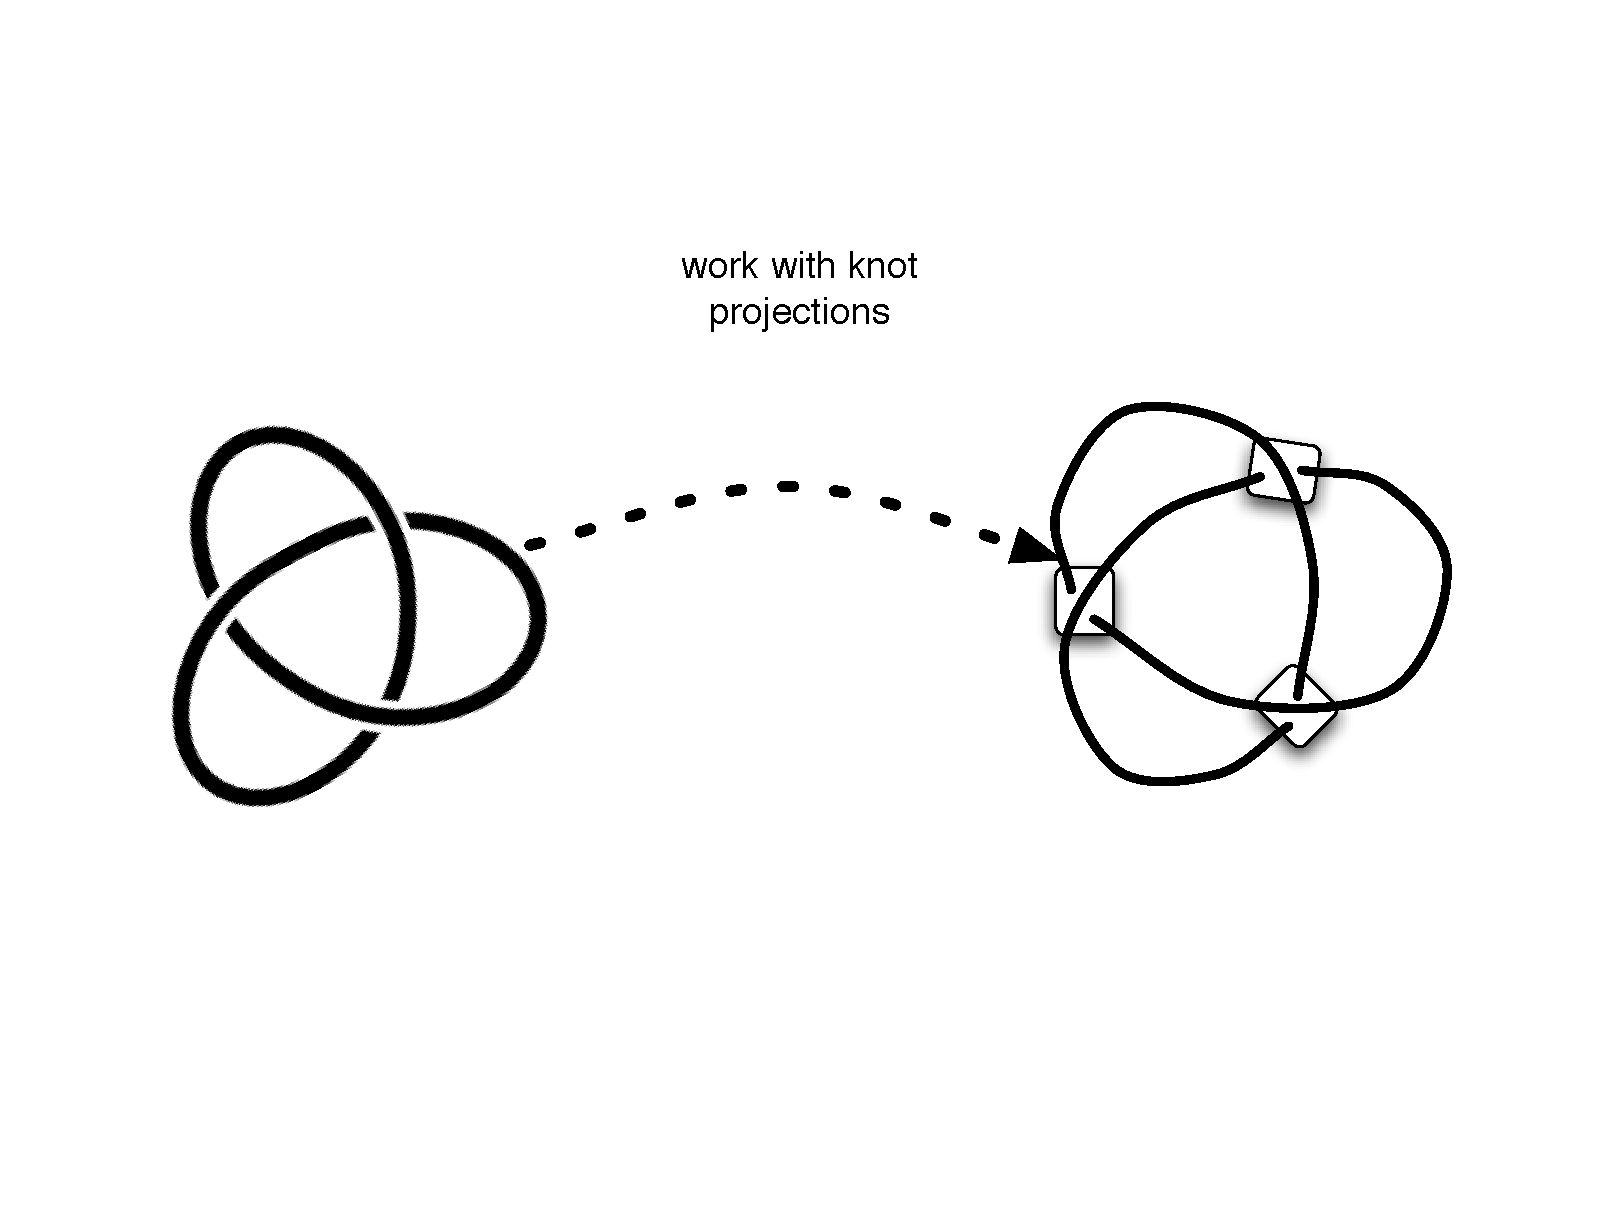
\includegraphics[viewport=20 200 810 480]{TrefoilMethodIllustrationStepOne21072006}}
    \caption{ Trefoil as projection }
\end{figure}
\end{frame}

\begin{frame}
  \frametitle{Trefoil as computing device}
  \framesubtitle{Crossings as circuits}
  \begin{figure}[tbp]
    \centering
    \scalebox{0.40}[0.400]{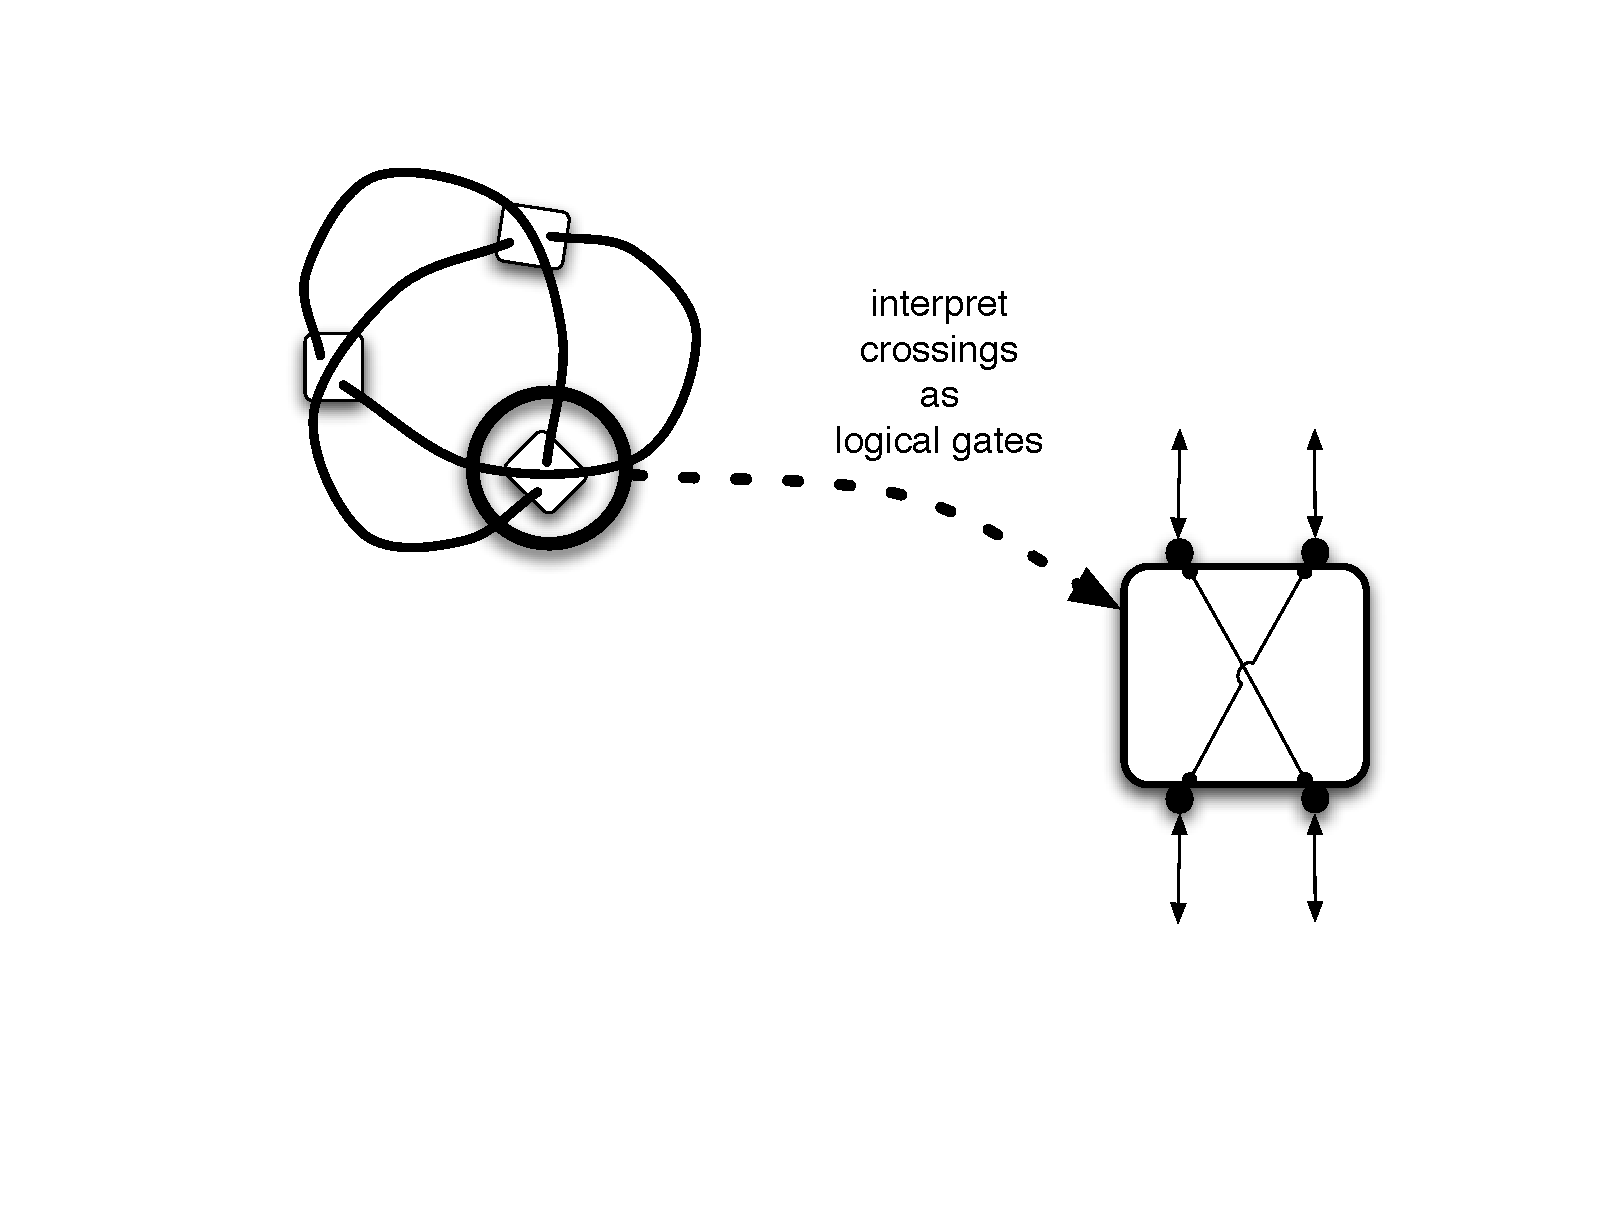
\includegraphics[viewport=30 200 810 500]{TrefoilMethodIllustrationStepTwo21072006}}
    \caption{ Crossings as circuits }
\end{figure}
\end{frame}

\begin{frame}
  \frametitle{Trefoil as computing device}
  \framesubtitle{Wiring it all together}
  \begin{figure}[tbp]
    \centering
    \scalebox{0.30}[0.300]{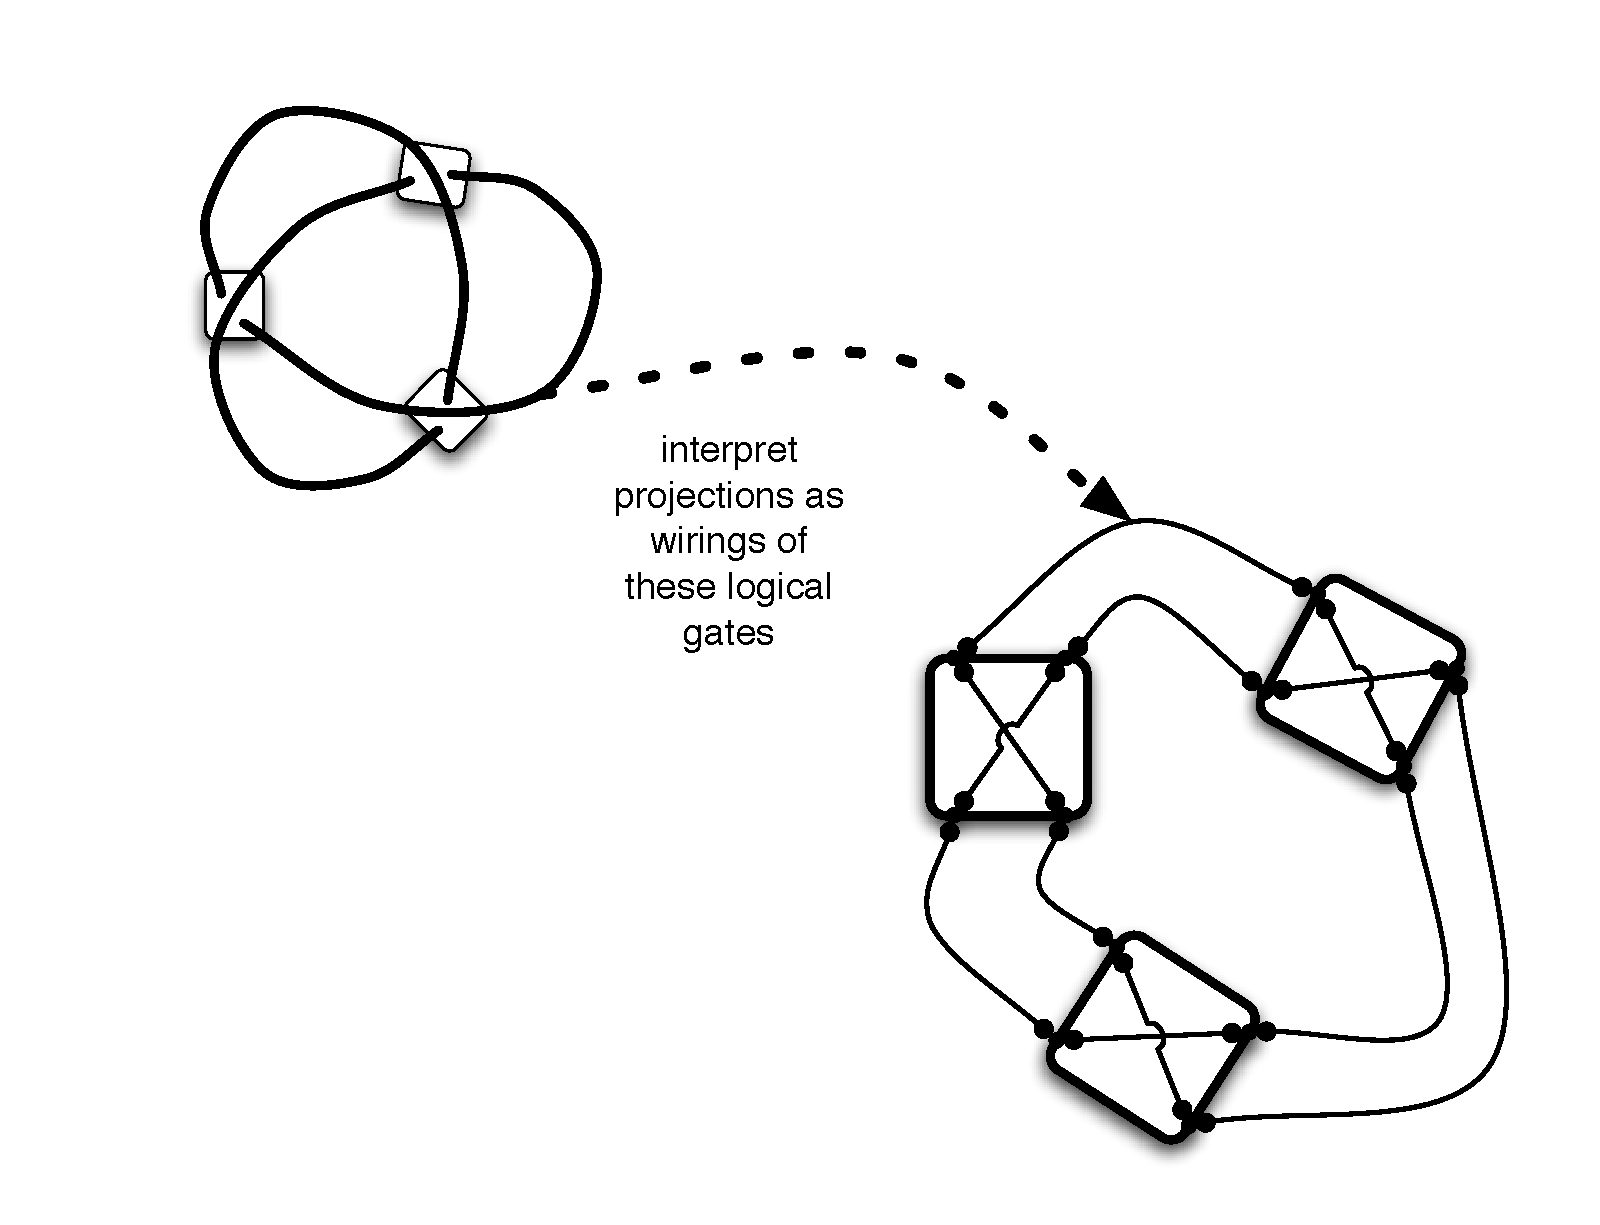
\includegraphics[viewport=30 30 810 550]{TrefoilMethodIllustrationStepThree21072006}}
    \caption{ Trefoil as device }
  \end{figure}
\end{frame}

\begin{frame}
  \frametitle{Crossing circuits}
  \begin{figure}[tbp]
    \centering
    \scalebox{0.27}[0.270]{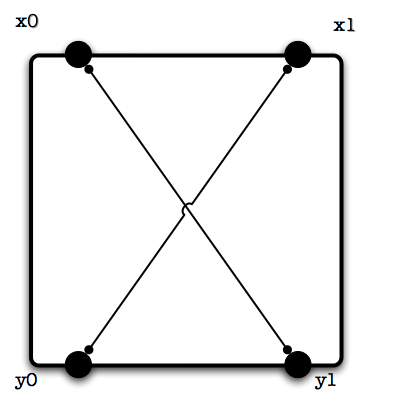
\includegraphics[viewport=0 0 390 360]{BasicCrossingCircuit}}
    %\caption{ Crossing circuit }
\end{figure}
\begin{eqnarray}
  \lefteqn{ C(x_0,x_1,y_0,y_1,u) := } \nonumber \\
  & & x_1?(s).y_0!(s).(C(x_0,x_1,y_0,y_1,u)|u!) \nonumber \\
  & & + y_0?(s).x_1!(s).(C(x_0,x_1,y_0,y_1,u)|u!) \nonumber \\
  & & + x_0?(s).u?.y_1!(s).(C(x_0,x_1,y_0,y_1,u)) \nonumber \\
  & & + y_1?(s).u?.x_0!(s).(C(x_0,x_1,y_0,y_1,u)) \nonumber
\end{eqnarray}
\end{frame}

\begin{frame}
  \frametitle{Wires and buffers}
  \begin{eqnarray}
    W(x,y) & := & (\nu \; n \; m)(Waiting(x,n,m) | Waiting(y,m,n)) \nonumber
  \end{eqnarray}

  \begin{eqnarray}
    % W(x_0,x_1) := x_0?(s).x_1!(s).W(x_0,x_1) + x_1?(s).x_0!(s).W(x_0,x_1) 
    \lefteqn{ Waiting(x,c,n) :=} \nonumber \\
    & & x?(v).(\nu \; m)(Cell(n,v,m) | Waiting(x,c,m)) \nonumber \\
    & & + c?(w).c?(c).Ready(x,c,n,w) \nonumber \\
    \lefteqn{ Ready(x,c,n,w) :=} \nonumber \\
    & & x?(v).(\nu \; m)(Cell(n,v,m) | Ready(x,c,m,w)) \nonumber \\
    & & + x!(w).Waiting(x,c,n) \nonumber
  \end{eqnarray}

  \begin{eqnarray}
    Cell(c,v,n) & := & c!(v).c!(n).0 \nonumber
  \end{eqnarray}
\end{frame}

\section{General encoding}
\begin{frame}
  \frametitle{Main theorem}
  \begin{equation}{\mbox{Main theorem: }}
    K_1 \sim K_2 \iff \meaningof{K_1} \simeq \meaningof{K_2} \nonumber
  \end{equation}
  
  Need to unpack

  \begin{itemize}
    \item $\meaningof{-} : Knots \to \pi$
      \begin{itemize}
        \item specify target language, $\pi$-calculus
        \item specify a source language, $Knots$
      \end{itemize}
    \item notion of equivalence, $\sim$, in $Knots$
    \item notion of equivalence, $\simeq$, in $\pi$-calculus
  \end{itemize}
\end{frame}

\subsection{Target language}
\begin{frame}
  \frametitle{Target language: $pi$ in 5}
  \framesubtitle{Syntax}
  \begin{grammar}
    \mbox{summation} & {N} & \bc & \Sigma_{i \in I} x_i.A_i \\
    \mbox{agent} & {A} & \bc & F \;| \; C \;| \; (\nu \; \vec{x})A \\
    \mbox{abstraction} & {F} & \bc & (\vec{x})P \;| \; (\nu \; \vec{x})F \\
    \mbox{concretion} & {C} & \bc & [\vec{x}]P \;| \; (\nu \; \vec{x})C \\
    \mbox{process} & {P,Q} & \bc & N \;| \;P|Q \;| \; (\nu \; \vec{x})P \\
                   & & \;| & X\langle \vec{y} \rangle \;| \; (\textsf{rec} \; X(\vec{x}).P)\langle \vec{y} \rangle                   
  \end{grammar} 

  \begin{eqnarray}
  x?(\vec{y}).P & \triangleq & x.(\vec{y})P \nonumber \\
  x!(\vec{y}).P & \triangleq & x.[\vec{y}]P \nonumber
\end{eqnarray}
\end{frame}

\begin{frame}
  \frametitle{Target language: $pi$ in 5}
  \framesubtitle{Structural equivalence}
  The {\em structural congruence}, $\equiv$, between processes is the
  least congruence closed with respect to alpha-renaming, satisfying
  AC for $|$ and $+$, $\pzero$  following axioms:
  \begin{enumerate}
  \item the scope laws:
    \begin{eqnarray}
      (\nu \; x)\pzero  & \equiv & \pzero, \nonumber\\
      (\nu \; x)(\nu \; x)P & \equiv & (\nu \; x)P, \nonumber\\
      (\nu \; x)(\nu \; y)P & \equiv & (\nu \; y)(\nu \; x)P, \nonumber\\
      P | (\nu \; x)Q & \equiv & (\nu \; x)(P|Q), \; \mbox{\textit{if} }x \not\in \freenames{P} \nonumber
    \end{eqnarray}
  \item
    the recursion law:
    \begin{eqnarray}
      (\textsf{rec} \; X(\vec{x}).P)\langle \vec{y} \rangle \equiv P\{\vec{y}/\vec{x}\}\{(\textsf{rec} \; X(\vec{x}).P)/X\} \nonumber
    \end{eqnarray}
  \end{enumerate}
\end{frame}

\begin{frame}
  \frametitle{Target language: $pi$ in 5}
  \framesubtitle{Operational semantics}
  \begin{mathpar}
    \inferrule* [Right=Comm] { |F| = |C| } { x.F \juxtap x.C \red F \circ C }
    \and \\
    \inferrule* [Left=Par] {{P} \red {P}'} {{{P} | {Q}} \red {{P}' | {Q}}}
    \and
    \inferrule* [Right=New] {{P} \red {P}'} {{\newp{{x}}{{P}}} \red {\newp{{x}}{{P}'}}}
    \and \\
    \inferrule* [Right=Equiv]{{{P} \scong {P}'} \andalso {{P}' \red {Q}'} \andalso {{Q}' \scong {Q}}}{{P} \red {Q}}
  \end{mathpar}
  \begin{equation}
    (\vec{y})P \circ (\nu \vec{v})[\vec{z}]Q \triangleq (\nu \vec{v})(P\{\vec{z}/\vec{y}\} | Q) \nonumber
  \end{equation}
  As usual, write $\wred$ for $\red^*$.
\end{frame}

\begin{frame}
  \frametitle{Target language: $pi$ in 5}
  \framesubtitle{Bisimulation}
  \begin{definition}
    An agent, $B$, occurs \emph{unguarded} in $A$ if it has an occurence
    in $A$ not guarded by a prefix $x$. A process $P$ is observable at
    $x$, written here $P \downarrow x$, if some agent $x.A$ occurs
    unguarded in $P$. We write $P \Downarrow x$ if there is $Q$ such
    that $P \wred Q$ and $Q \downarrow x$.
  \end{definition}
\end{frame}

\begin{frame}
  \frametitle{Target language: $pi$ in 5}
  \framesubtitle{Bisimulation}
  \begin{definition}
    % \label{def.bbisim}
    A \emph{barbed bisimulation} is a symmetric binary relation 
    ${\mathcal S}$ between agents such that $P\rel{S}Q$ implies:
    \begin{enumerate}
    \item If $P \red P'$ then $Q \wred Q'$ and $P'\rel{S} Q'$.
    \item If $P\downarrow x$, then $Q\Downarrow x$.
    \end{enumerate}
    $P$ is barbed bisimilar to $Q$, written
    $P \simeq Q$, if $P \rel{S} Q$ for some barbed bisimulation ${\mathcal S}$.
  \end{definition}
\end{frame}

\begin{frame}
  \frametitle{Shape of the encoding} 

  Now we are in a position to unpack the general shape of the
  encoding. It's just a parallel composition of crossings and wires
  wired up to respect the graph underlying the knot projection

  \begin{eqnarray}
    \lefteqn{\meaningof{K} =} \nonumber \\
    & & (v_0 ... v_{4n-1})( \Pi_{i = 0}^{n-1} (\nu \; u)\meaningof{C(i)}(v_{4i},...,v_{4i+3},u) \nonumber \\
    & & \; \; \; \; \; \; \; \; \; \; \; \; \; \; \; \; \; \; | \Pi_{i = 0}^{n-1} W(v_{\omega(i,0)},v_{\omega(i,1)})|W(v_{\omega(i,2)},v_{\omega(i,3)}) ) \nonumber
    \end{eqnarray}
\end{frame}

\subsection{Source language}
\begin{frame}
  \frametitle{A (very) little knot theory}    
  \begin{itemize}
    \item A knot is an embedding of the circle into $\Real^3$
    \item Two knots, $K_1$ and $K_2$ can be composed, $K_1 \# K_2$ by
      cutting each and fusing the respective ends together
    \item A prime knot cannot be represented as the composition of knots
    \item We can work with knot projections because of a well-known
      theorem stating that knots are ambient isotopic iff you can
      convert the projection of one into the projection of the other
      via a sequence of the Reidemeister moves.
  \end{itemize}
  \begin{figure}[tbp]
    \centering
    \scalebox{0.30}[0.300]{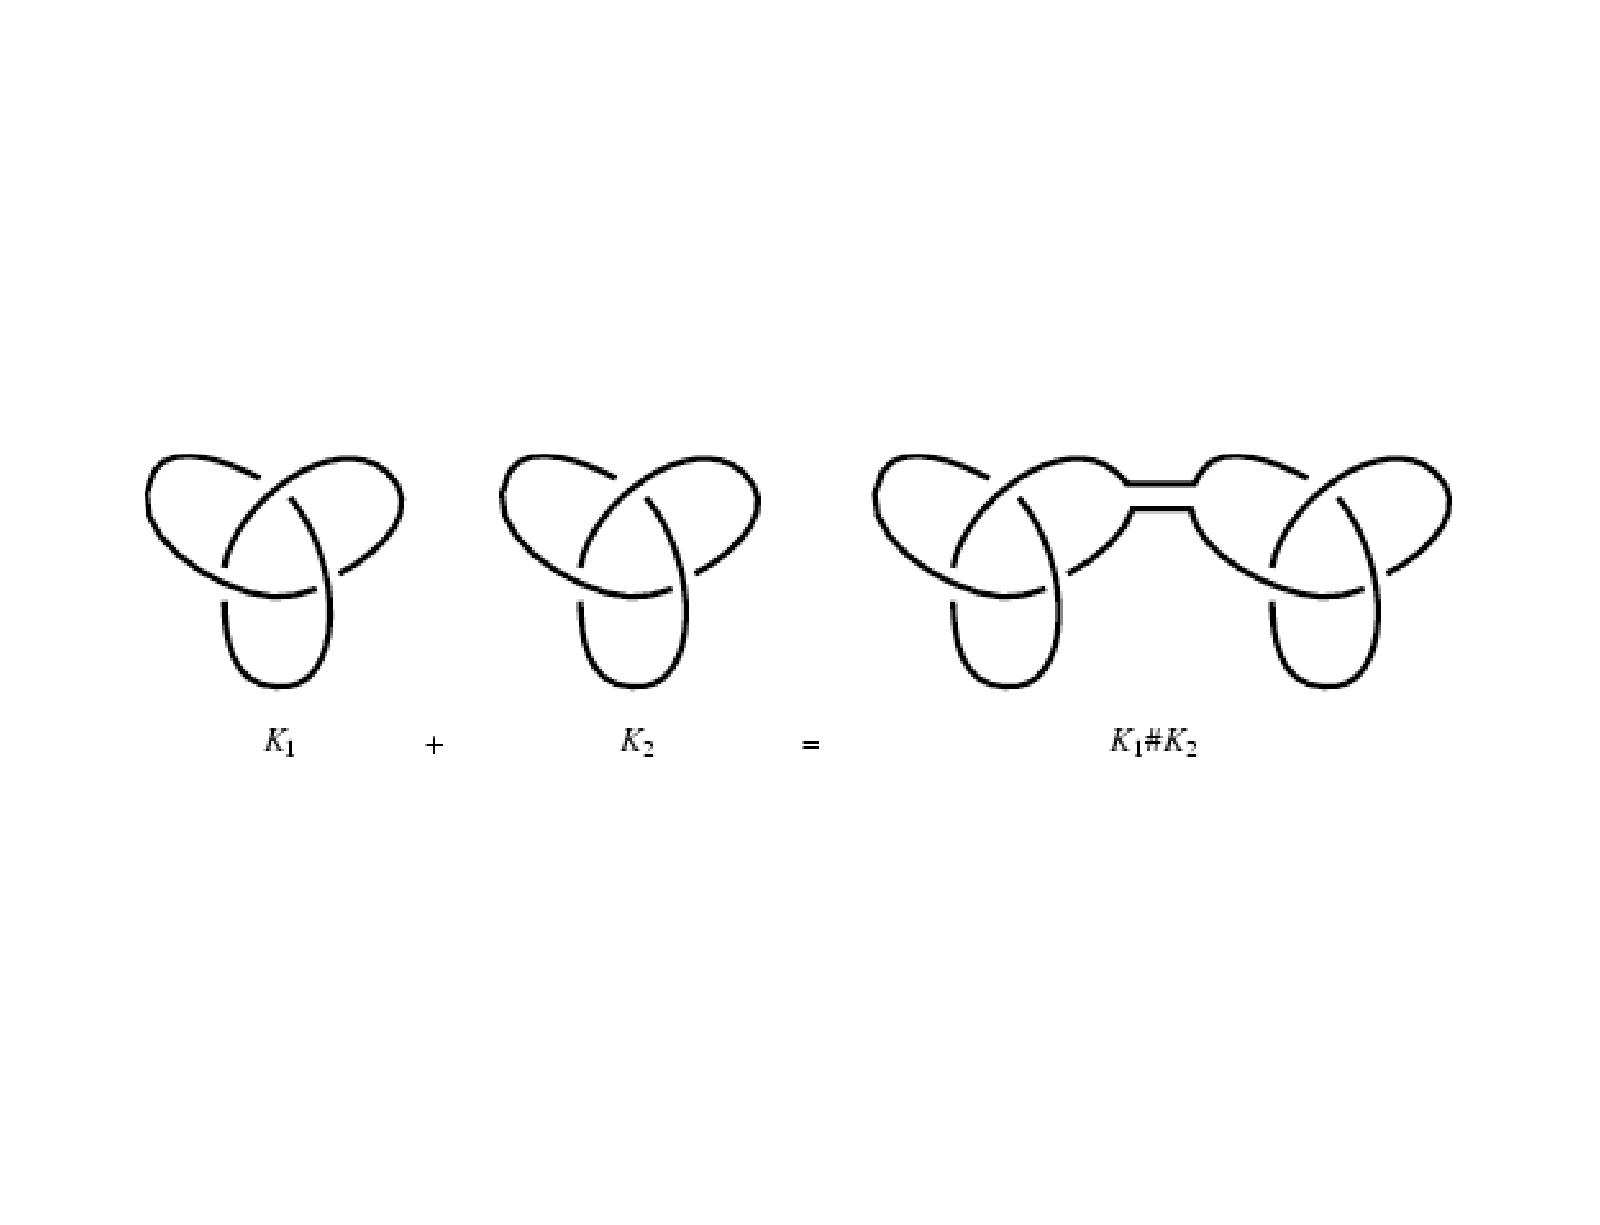
\includegraphics[viewport=30 30 810 350]{KnotSum}}
    \caption{ Trefoil as device }
  \end{figure}
\end{frame}

\begin{frame}
  \frametitle{Reidemeister moves}    
  In `digitizing' knots by working with their projections we obtained
  another notion of equivalence: the Reidemeister moves
  \textit{operationalize} ambient isotopy.
  \begin{figure}[tbp]
    \centering
    \scalebox{0.25}[0.250]{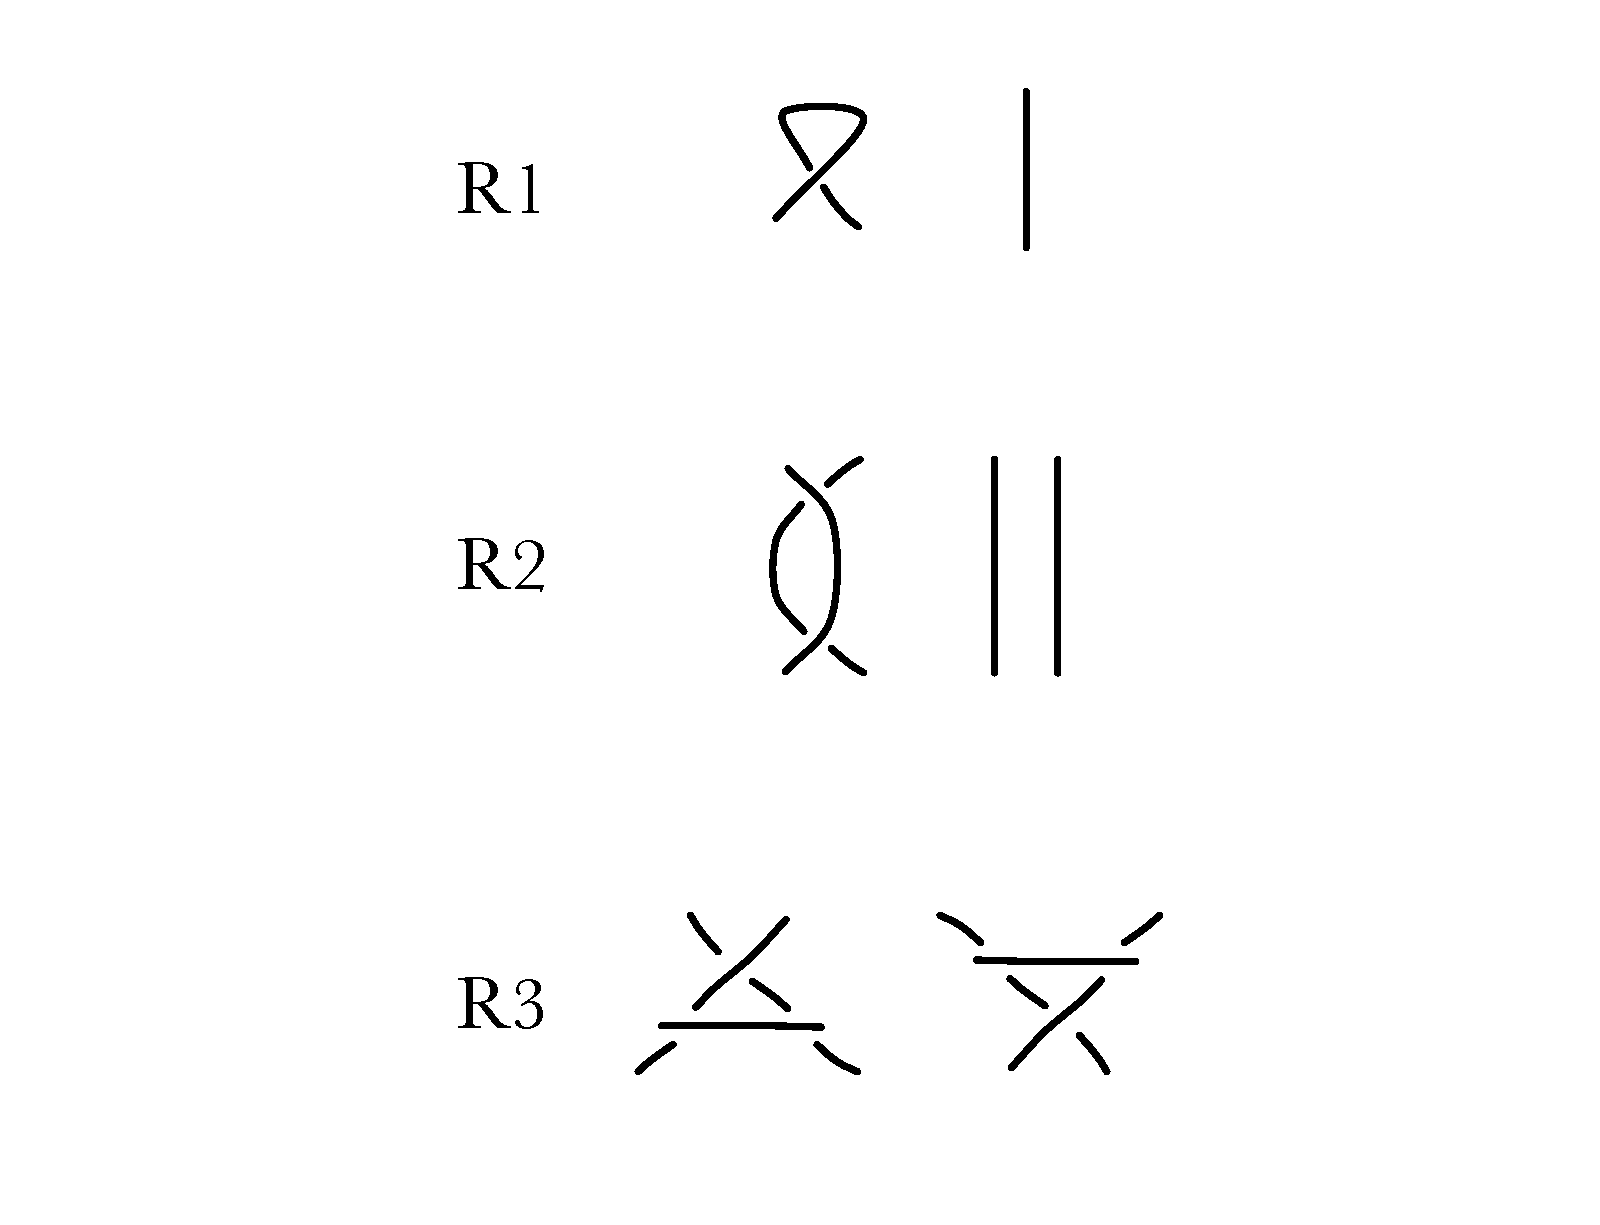
\includegraphics[viewport=0 75 700 525]{ReidemeisterMoves12321072006}}
    \caption{ Reidemeister moves }
  \end{figure}
\end{frame}

\begin{frame}
  \frametitle{Source language}
  Candidates for a language for representing knots as input to the encoding
  \begin{itemize}
    \item Dowker-Thistlethwaite codes
      \begin{itemize}
        \item \textit{unique} for prime knots
      \end{itemize}
    \item John Horton Conway's Tangle Calculus a.k.a. Knotation
      \begin{itemize}
        \item Representation theorem for rational tangles
      \end{itemize}
    \item Signed planar graphs
  \end{itemize}
\end{frame}

\begin{frame}
  \frametitle{DT-codes by example}
  \begin{figure}[tbp]
    \centering
    \scalebox{0.4}[0.400]{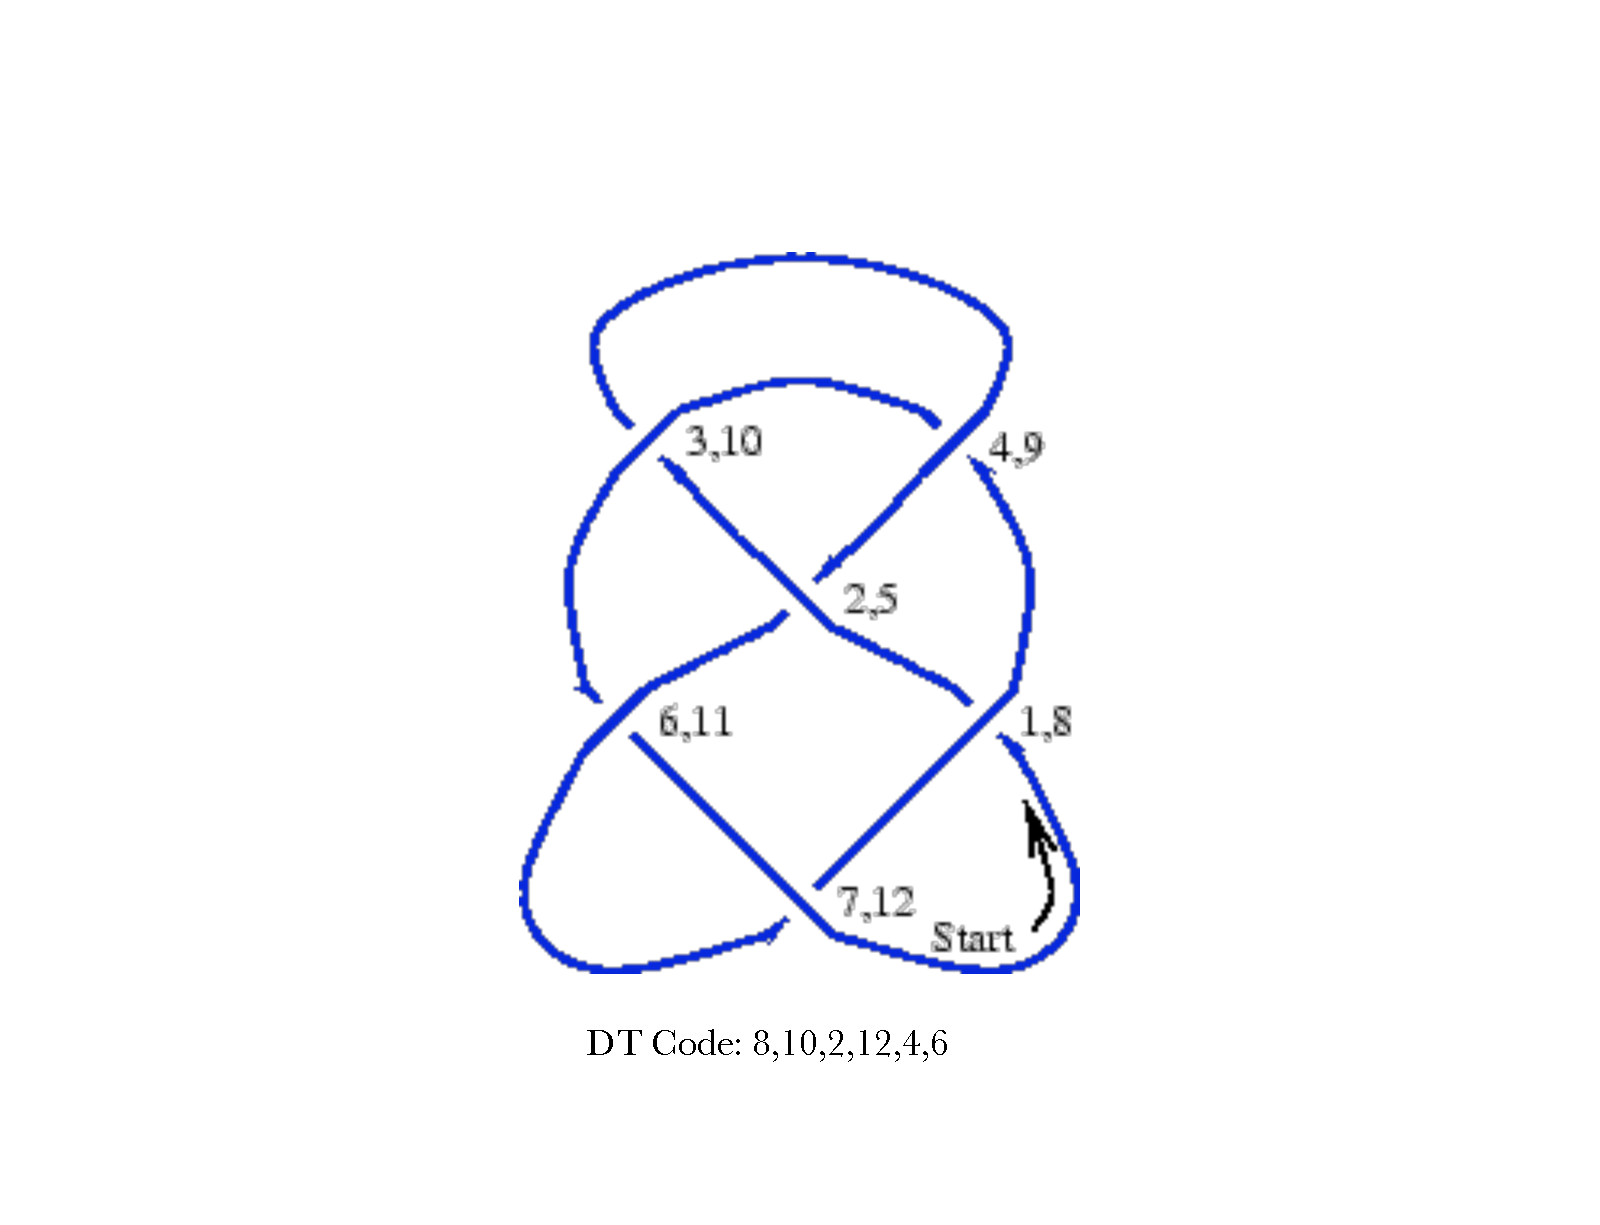
\includegraphics[viewport=0 125 850 425]{DTCodeExample}}
    \caption{ DT-code example }
  \end{figure}
\end{frame}

\begin{frame}
  \frametitle{DT-codes}
  \framesubtitle{Just the facts}
  \begin{itemize}
    \item Provides a bijective map, $DT$, between 
      \begin{itemize}
        \item $\{ i : odd(i), 1 \leq i \leq 2n \}$
        \item $\{ i : even(i), 2 \leq i \leq 2n \}$
      \end{itemize}
    \item Connects $C(i)$ to 
      \begin{itemize}
        \item $C(i-1)$ 
        \item $C(i+1)$ 
        \item $C(DT^{-1}(DT(i)-1))$
        \item $C(DT^{-1}(DT(i)+1))$ 
      \end{itemize}
    \item Provides enough information to say whether $i$-path or
      $DT(i)$-path is the over-crossing
  \end{itemize}
\end{frame}

\begin{frame}
  \frametitle{DT-codes}
  \framesubtitle{Wiring algorithm}
%  \begin{lstlisting}
   let DTWiring i dt dti knot acc = 
     if (i <= (numCrossings knot)) 
     then 
       let ic = (2*i - 1) in 
         (DTWiring 
	      (i+1) dt knot 
	    (union  	    
	       acc 
	       [ W(x1(C(knot,ic)), 
		   (if (over dt ic-1) then y0 else y1)); 
	         W(y0(C(knot,ic)), 
		   (if (over dt ic+1) then x1 else x0)); 
	         W(x0(C(knot,ic)), 
		   (if (over dt (dti ((dt i)-1))) then y0 else y1)); 
	         W(y1(C(knot,ic)), 
		   (if (over dt (dti ((dt i)+1))) then x1 else x0)) ])) 
     else acc
%     \end{lstlisting}
\end{frame}

\section{Main theorem: proof sketch}

\begin{frame}
  \frametitle{Supporting definitions}
  \begin{definition}
    We will say that the encoding of a knot is \textit{alive} as long
    as it is firing. If it ever ceases to push signal through, then it
    is \textit{dead}.

    We can ascertain an upperbound on initial signal that guarantees
    liveness of the encoding. Surely, $2\#(K)$ will guarantee the
    liveness of the encoding. More declaratively, we simply demand
    that $ \meaningof{K} | initialSignal$ be live before we are willing to
    admit it as a representation of the knot.
  \end{definition}
\end{frame}

\subsection{Forward direction}

\begin{frame}
  \frametitle{Ambient isotopic knots have bisimilar encodings}
  \begin{itemize}
  \item Since $K_1 \sim K_2$ we know there is a sequence of
    Reidemeister moves converting $K_1$ to $K_2$
  \item Each move corresponds to a bisimilarity preserving
    transformation on the process encoding
  \end{itemize}
\end{frame}

\begin{frame}
  \frametitle{R-move interfaces}
  \begin{itemize}
  \item For the following two lemmas we have to keep the
    \textit{interface}, i.e. splice points, of the left and right hand
    sides of the R-move the same. So, for R1L and R2L we must restrict
    the ports that are not the splice points.
  \item One way to address this is to embed the restrictions into the
    encodings of R1L and R2L. Algebraically,
    \begin{eqnarray}
      \lefteqn{\meaningof{R1L}(y0,y1) =} \nonumber \\
      & & (\nu \; x_{0} \; x_{1}) ((\nu \; u)C(x_{0},x_{1},y_{0},y_{1},u) | W(x_{0},x_{1})) \nonumber \\
      \lefteqn{\meaningof{R2L}(x_{00},x_{01},x_{10},x_{11}) =} \nonumber \\
      & & (\nu \; y_{00},y_{01},y_{10},y_{11},)((\nu \; u_{0})C(x_{00},x_{01},y_{00},y_{01},u{0}) \nonumber \\
      & & | W(y_{00},y_{11}) | W(y_{01},y_{10}) | (\nu \; u_{1})C(x_{10},x_{11},y_{10},y_{11},u_1)) \nonumber
    \end{eqnarray}
    \item Technically it will be convenient to break out the restrictions
  \end{itemize}
\end{frame}

\begin{frame}
  \frametitle{R-move interfaces}
  \framesubtitle{Example}
  \begin{figure}[tbp]
    \centering
    \scalebox{0.30}[0.300]{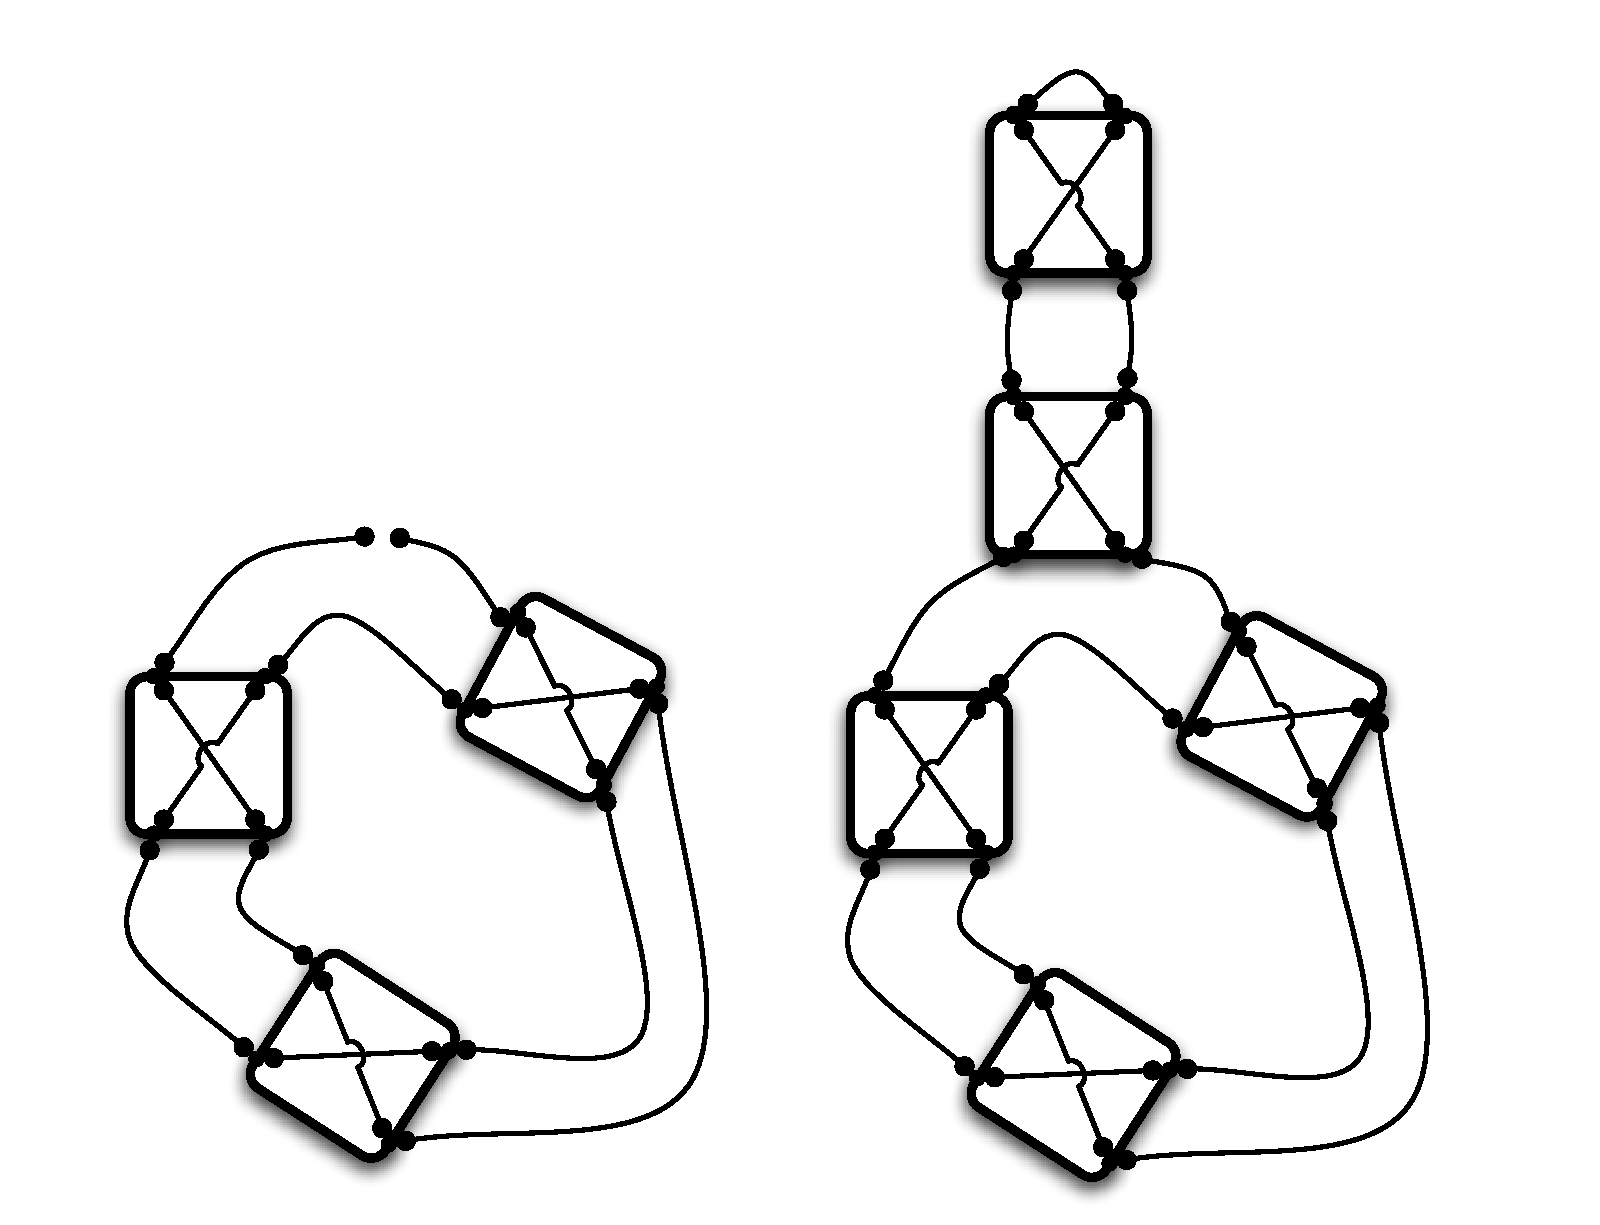
\includegraphics[viewport=30 30 810 520]{TrefoilMethodIllustrationWithFingerMove221072006}}
    \caption{ Reidemeister move and context }
  \end{figure}
\end{frame}

% \begin{frame}
%   \frametitle{R-move interfaces, cont.}
%   , and so we define $\meaningof{R1L}_{-\nu}$ and $\meaningof{R2L}_{-\nu}$ by
%   \begin{eqnarray}
%     \meaningof{R1L}(y_0,y_1) =: \meaningof{R1L}_{-\nu}(x_0,x_1,y_0,y_1) \nonumber \\
%     \meaningof{R2L}(x_{00},x_{01},x_{10},x_{11}) =: (\nu \; y_{00},y_{01},y_{10},y_{11},)\meaningof{R2L}_{-\nu}(\vec{x},\vec{y}) \nonumber
%   \end{eqnarray}
%   and then abuse notation by taking the {-\nu} meaning as the default.
% \end{frame}

\begin{frame}
  \frametitle{R-moves: context lemma}
  
  $\forall i \in \{ 1, 2, 3 \}$ \; if $K_{1}
  \stackrel{Ri}{\rightarrow} K_{2}$ then there exists a context $M$
  and (possibly empty) vector of distinct names, $\vec{w}$ s.t.
  \begin{eqnarray}
    (\nu \; \vec{w})\meaningof{K_{1}}\langle v:w\rangle & = & (\nu \; \vec{w})M[ \meaningof{RiL} ] \nonumber \\
    \meaningof{K_{2}} & = & M[ \meaningof{RiR} ] \nonumber
  \end{eqnarray}

  Pf: This follows directly from the definition of the encoding.

\end{frame}

\begin{frame}
  \frametitle{R-moves: substitution lemma}
  We argue that $RiL$ is bisimilar to $RiR$ in the context of a live encoding.That is if
  \begin{itemize}
    \item $\meaningof{K} | initialSignal$ is alive, and
    \item $\meaningof{K} | initialSignal = C[ \meaningof{RiL} ]$
  \end{itemize}

  then we can substitute $\meaningof{RiR}$ in its place without change of behavior, i.e.
  
  \begin{eqnarray}
    \forall i \in \{ 1, 2, 3 \} \; (\nu \; \vec{w})C[ \meaningof{RiL} ] & \simeq & C[ \meaningof{RiR} ] \nonumber
  \end{eqnarray}
\end{frame}

\begin{frame}
  \frametitle{R-moves as bisimilarity preserving xforms}
  \begin{figure}[tbp]
    \centering
    \scalebox{0.30}[0.300]{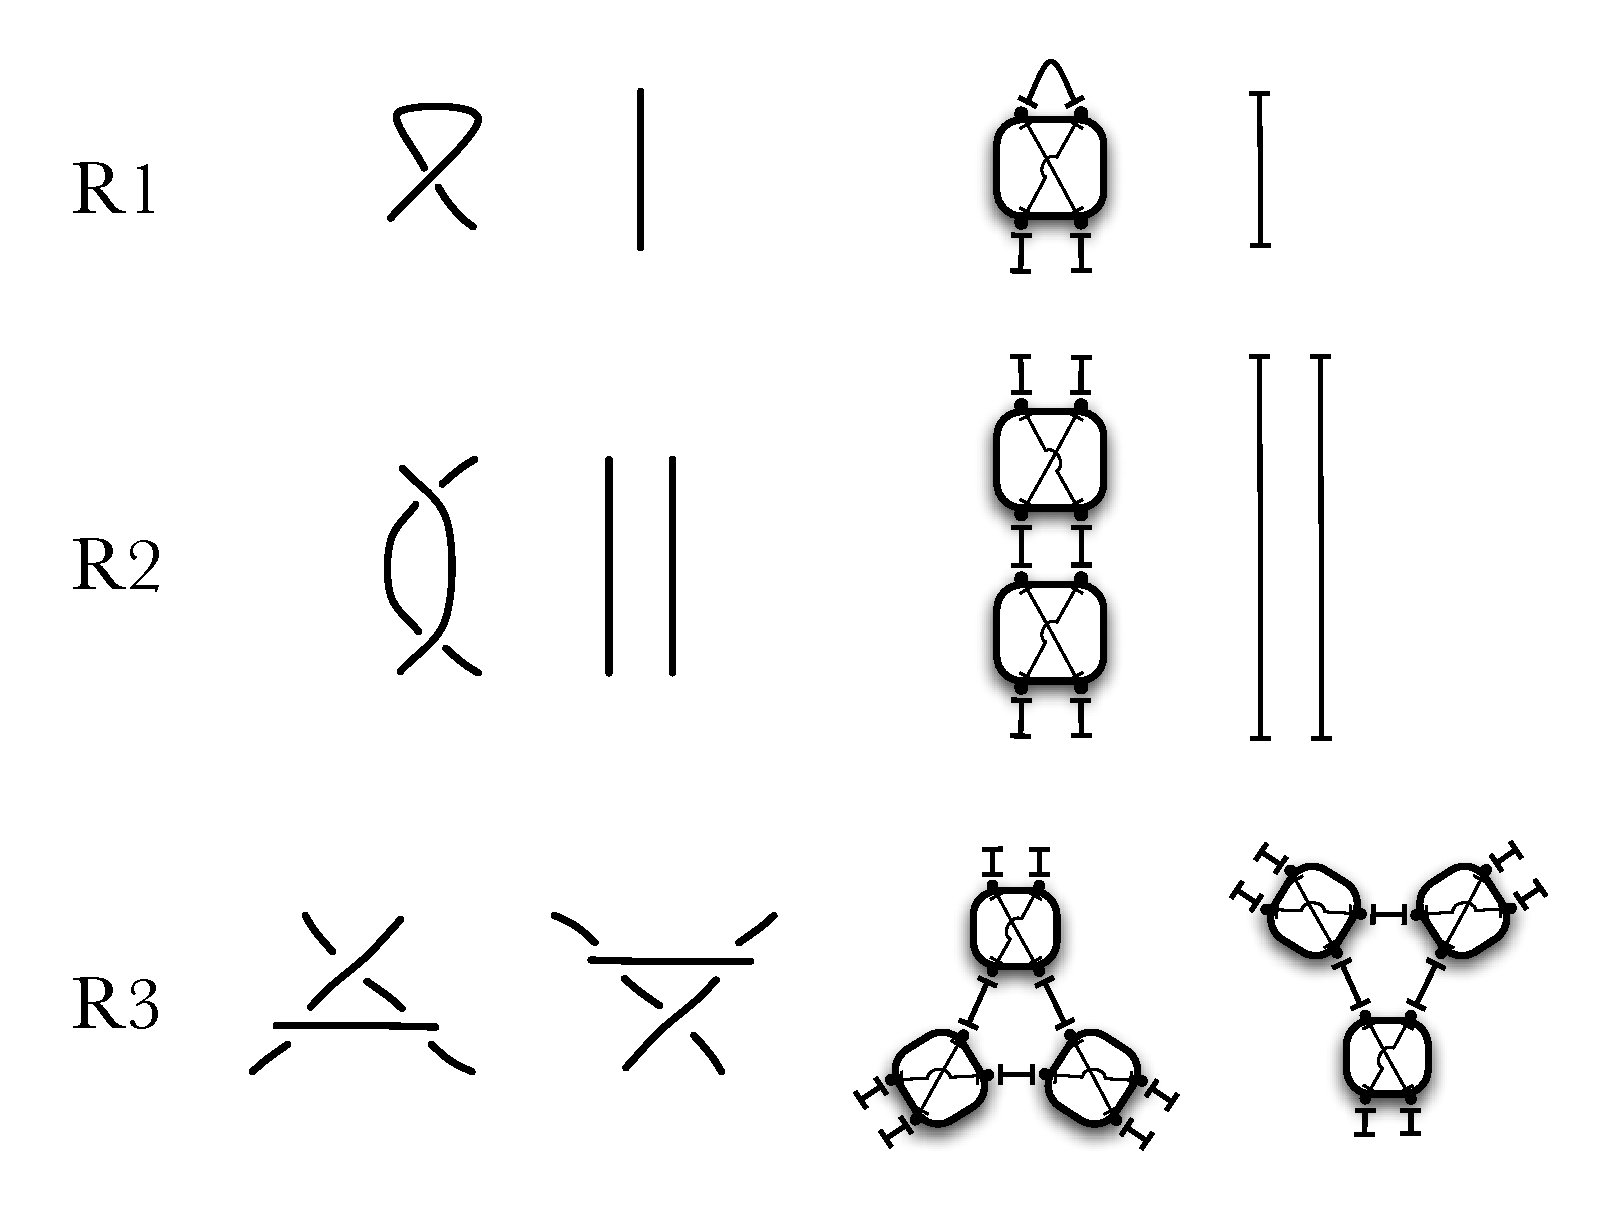
\includegraphics[viewport=30 30 810 550]{ReidemeisterMovesAsCircuits21072006}}
    \caption{ Reidemeister moves as bisimilar processes }
  \end{figure}
\end{frame}

\begin{frame}
  \frametitle{R-moves: technical meaning of forward direction}
  
  \begin{itemize}
    \item $\meaningof{K_{1}}$ is an abstraction in $4\#(K_{1})$
    \item $\meaningof{K_{2}}$ is an abstraction in $4\#(K_{2})$
    %\item w.l.o.g. assume $\#(K_{1}) \leq \#(K_{2})$
    \item let $\#_{Min}(K) := min\{\#(K') : K' \sim K \}$
  \end{itemize}
  
  We assert that there is an $4\#_{Min}(K_1) \leq n \leq 4*max\{ \#(K_1),
  \#(K_2) \}$ for any vector of names, $\vec{v}$, s.t.

  \begin{itemize}
  \item $|\vec{v}| = n$,
  \item $v[i] \neq v[j] \iff i \neq j $
  \item there exists two vectors of names, $\vec{w_1}, \vec{w_2}$,
    also all distinct, s.t.
    \begin{eqnarray}
      (\nu \; \vec{w_1})\meaningof{K_{1}}\langle \vec{v}:\vec{w_1} \rangle & \simeq & (\nu \; \vec{w_2})\meaningof{K_{2}}\langle \vec{v}:\vec{w_2} \rangle \nonumber
    \end{eqnarray}
    with $|\vec{w_i}| = 4\#(K_{i}) - n$.
  \end{itemize}    

\end{frame}

 \begin{frame}
   \frametitle{R-moves: technical meaning of forward direction}
   \framesubtitle{Strengthening} 

   Let
  
   \begin{eqnarray}
     \lefteqn{L_C(\meaningof{K}\langle \vec{u} \rangle, \vec{v}) :=} \nonumber \\
     & & \{ (\nu \; u)C(\vec{z}) : \exists P \; \meaningof{K}\langle \vec{u} \rangle = (\nu \; u)C(\vec{z}) | P \} \nonumber \\
     \lefteqn{L_W(\meaningof{K}\langle \vec{u} \rangle, \vec{v}, \vec{w}) :=} \nonumber \\
     & & \{ W(a,b) : \exists P \; \meaningof{K}\langle \vec{u} \rangle = W(a,b) | P, a,b \in \vec{v}, a, b \not\in \vec{w} \} \nonumber \\
     \lefteqn{L(\meaningof{K}\langle \vec{u} \rangle, \vec{v}, \vec{w}) :=} \nonumber \\
     & & \Pi_{C \in L_{c}(\meaningof{K}\langle \vec{u} \rangle, \vec{v})}C | \Pi_{W \in L_{W}(\meaningof{K}\langle \vec{u} \rangle, \vec{v}, \vec{w})} W \nonumber
   \end{eqnarray}

   we also have

   \begin{eqnarray}
     L(\meaningof{K_{1}}\langle \vec{v}:\vec{w_1} \rangle,\vec{v},\vec{w_1}:\vec{w_2}) = L(\meaningof{K_{2}}\langle \vec{v}:\vec{w_2} \rangle,\vec{v},\vec{w_1}:\vec{w_2}) \nonumber
   \end{eqnarray}

 \end{frame}

\begin{frame}
  \frametitle{Forward direction: moral content} 

  \begin{itemize}
  \item When the knots are ambient isotopic the encodings
    \textit{share} a set of crossings and wires at least as big as a
    minimal crossing representative of the isotopy class.
  \item And the other parts are R-move complications of wires that
    would complete the knot from shared core -- hidden under restriction.
  \end{itemize}

\end{frame}

\begin{frame}
  \frametitle{R-moves: one step lemma}
  If $K_{1}$ is one R-move away from $K_{2}$ then 

  \begin{eqnarray}
    \meaningof{K_{1}}\langle v \rangle & \simeq & (\nu \; w)\meaningof{K_{2}}\langle v:w \rangle \nonumber
  \end{eqnarray}

  This follows directly from the context and substitution lemmas.
\end{frame}

\begin{frame}
  \frametitle{R-moves: iteration of one-step lemma} 
  \begin{itemize}
  \item Even if you have a simplifying step followed by a complicating
    step, you can iterate the one-step lemma, mimicking the
    Reidemeister theorem.

  \item The reason is that crossings in a complicating step can never
    be involved in any other part of the context. They are effectively
    hidden behind the interface defined by the simplified side of the
    R-move.
\end{itemize}
\end{frame}

\begin{frame}
  \frametitle{R-moves: R1L -> R1R; R2R -> R2L} 
  \framesubtitle{R1L -> R1R}
  \begin{itemize}
   \item The R1L $\to$ R1R step means we have a context $M$ such that
     \begin{eqnarray}
       (\nu \; x_0 \; x_1)\lefteqn{\meaningof{K_{1}}\langle \vec{v_0}:x_0 : x_1 \rangle} \nonumber \\
       & & = (\nu \; x_0 \; x_1)M[ \meaningof{R1L} ] \nonumber \\
       & & \simeq M[ \meaningof{R1R} ] \nonumber \\
       & & = \meaningof{K_{2}}\langle \vec{v_0} \rangle \nonumber
     \end{eqnarray}
   \end{itemize}
 \end{frame}

 \begin{frame}
   \frametitle{R-moves: R1L -> R1R; R2R -> R2L, cont.} 
   \framesubtitle{R2R -> R2L}
   \begin{itemize}
   \item The R2R $\to$ R2L step means we have a context $M'$ such that
     \begin{eqnarray}
       (\nu \; y_{00} \; y_{01} \; y_{10} \; y_{11})\lefteqn{\meaningof{K_{3}}\langle \vec{v_1}:y_{00} : y_{01} : y_{10} : y_{11} \rangle} \nonumber \\
       & & = (\nu \; y_{00} \; y_{01} \; y_{10} \; y_{11})M'[ \meaningof{R2L} ] \nonumber \\
       & & \simeq M'[ \meaningof{R1R} ] \nonumber \\
       & & = \meaningof{K_{2}}\langle \vec{v_1} \rangle \nonumber
     \end{eqnarray}
   \end{itemize}
 \end{frame}

 \begin{frame}
   \begin{itemize}
     \item We emphasize $\vec{v_0}, \vec{v_1}$ are just lists of distinct names with
       \begin{itemize}
         \item $|\vec{v_0}| = |\meaningof{K_{2}}| = |\vec{v_1}|$
       \end{itemize}
     \item so, pick $\vec{v_0} = \vec{v_1}$, dropping subscript, to conclude 
     \begin{eqnarray}
       \lefteqn{(\nu \; x_0 \; x_1)\meaningof{K_{1}}\langle \vec{v}:x_0 : x_1 \rangle \simeq} \nonumber \\
       & & (\nu \; y_{00} \; y_{01} \; y_{10} \; y_{11} )\meaningof{K_{3}}\langle \vec{v}:y_{00} : y_{01} : y_{10} : y_{11} \rangle \nonumber
     \end{eqnarray}
     \item with $\meaningof{K_{2}}\langle \vec{v} \rangle$ forming the shared core
   % \item hence $x_0,x_1$ do not occur free in $\vec{v}:y_{00} : y_{01} : y_{10} : y_{11}$,
%      and $y_{00}, y_{01}, y_{10}, y_{11}$ do not occur free in $\vec{v}:x_0 : x_1$
%    \item applying scope extrusion, twice, therefore yields the desired result.
   \end{itemize}
 \end{frame}

\subsection{Reverse direction}

\begin{frame}
  \frametitle{Bisimilar encodings come from isotopic knots} Strategy:
  assume encodings are bisimilar but knots not ambient isotopic and
  derive contradiction.
  \begin{itemize}
  \item W.l.o.g. demand knots be given in minimal crossing projections
  \item If crossing numbers are different then free names differ --
    contradicting bisimilarity
  \item Therefore crossing numbers must be the same
  \begin{itemize}
  \item $\Pi_{i=0}^{n-1} \meaningof{C(i)}(...) | \Pi_{i=0}^{n-1} W(...)|W(...) \simeq \Pi_{j=0}^{n-1} \meaningof{C(j)}(...) | \Pi_{j=0}^{n-1} W'(...)|W'(...)$
  \item $\Rightarrow \Pi_{i=0}^{n-1} W(...)|W(...) \simeq \Pi_{j=0}^{n-1} W'(...)|W'(...)$
  \item If any of these wires differ, then there is a distinguishing
    barb
  \item But, if none of them differ the knots must be ambient isotopic
    because their respective sets of crossings are wired identically -- contradiction
  \end{itemize}
  \end{itemize}
\end{frame}

\section{Conclusions and future work}

\begin{frame}
  \frametitle<presentation>{Conclusions}

  % Keep the summary *very short*.
  \begin{itemize}
  \item
    \alert{Computational calculi} constitute a reasonable new source of invariants.
  \item
    \alert{Bisimulation} is a proof method ready for wider exploitation.
  \item
   A first step towards another way to think about \alert{space as behavior}.
  \end{itemize}
  
  % The following outlook is optional.
  % \vskip0pt plus.5fill
%   \begin{itemize}
%   \item
%     Some things we haven't said
%     \begin{itemize}
%     \item
%       Knot sum has a direct representation in this encoding
%     \item
%       Kauffman bracket has a direct representation in this encoding
%     \end{itemize}
%     \item Future developments
%       \begin{itemize}
%         \item Applications to biology -- protein folding
%         \item Approach generalizes to give a direct representation of \textit{spin networks}
%       \end{itemize}
%   \end{itemize}
\end{frame}

\begin{frame}
  \frametitle<presentation>{Future work}

  % Keep the summary *very short*.
%   \begin{itemize}
%   \item
%     \alert{Computational calculi} constitute a reasonable new source of invariants.
%   \item
%     \alert{Bisimulation} is a proof method ready for wider exploitation.
%   \item
%    A first step towards another way to think about \alert{space as behavior}.
%   \end{itemize}
  
%   % The following outlook is optional.
%  \vskip0pt plus.5fill
  \begin{itemize}
  \item
    Some things we haven't said
    \begin{itemize}
    \item
      Knot sum has a direct representation in this encoding
    \item
      Kauffman bracket has a direct representation in this encoding
    \end{itemize}
    \item Applications and future developments
      \begin{itemize}
      \item Structure of knots now susceptible to inspection via
        Hennessy-Milner logics
      \item Applications to biology -- protein folding
      \item Approach generalizes to give a direct representation of \textit{spin networks}
      \end{itemize}
  \end{itemize}
\end{frame}

% \section*{Backup}
% \begin{frame}
%   \frametitle{Knotation}
%   \begin{figure}[tbp]
%     \centering
%     \scalebox{0.4}[0.400]{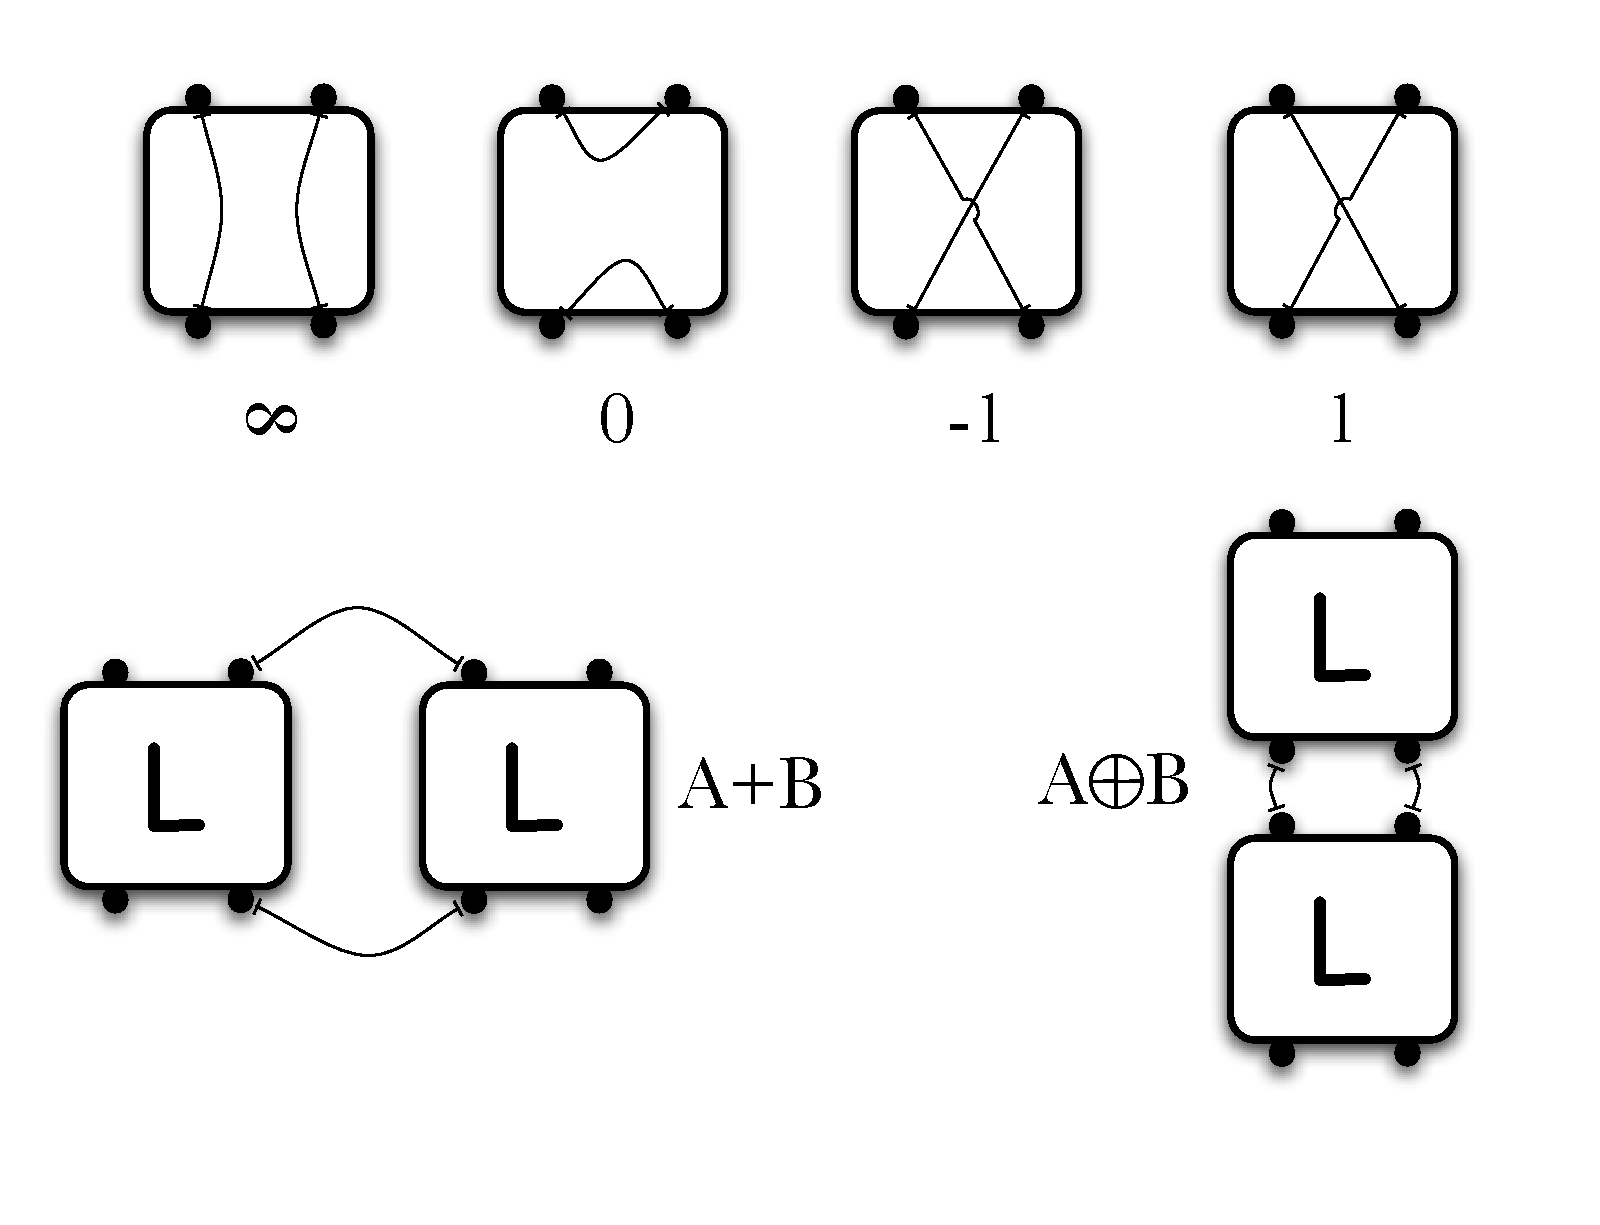
\includegraphics[viewport=0 175 950 525]{KnotationElementsWithOperations}}
%     \caption{ Knotation elements }
%   \end{figure}
% \end{frame}

% \begin{frame}
%   \frametitle{Knotation}
%   \framesubtitle{Just the facts}
%   \begin{itemize}
%   \item Knots can be named by assembling rational tangles (elements or
%     sums of a certain form) into tetravalent graphs called
%     polyhedra
%   \item Bangert has devised a class of univeral polyhedra the positions of which
%     are filled only with elements
%   \end{itemize}
% \end{frame}

% \begin{frame}
%   \frametitle{Universal polyhedron}
%   \begin{figure}[tbp]
%     \centering
%     \scalebox{0.3}[0.300]{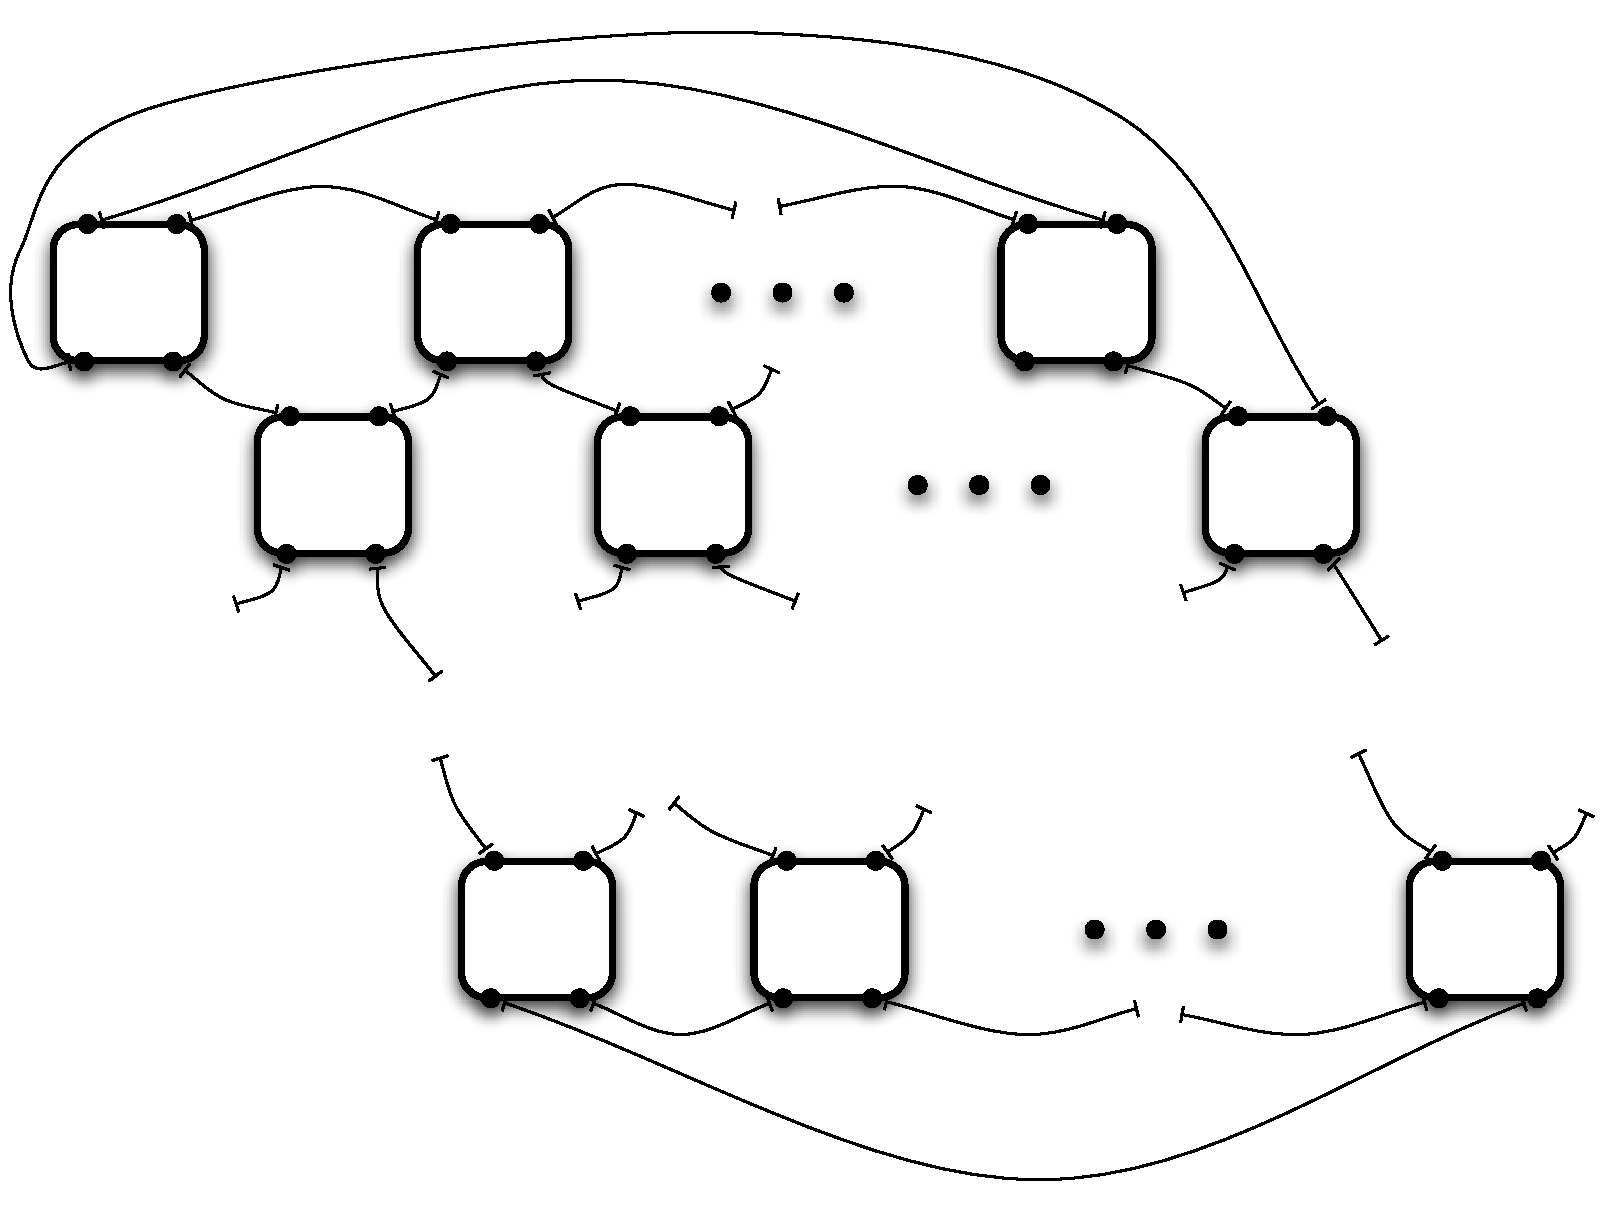
\includegraphics[viewport=0 50 950 525]{KnotationElementsUniversalPolyhedra}}
%     \caption{ Universal polyhedra }
%   \end{figure}
% \end{frame}

\end{document}


